\documentclass{article}
\usepackage[utf8]{inputenc}
\usepackage{amsfonts}
\usepackage{amsmath}
\renewcommand{\labelitemii}{$\circ$}
%% Custom commands
\newcommand{\E}[1]{\langle #1 \rangle} % shortcut for expectation
\newcommand{\norm}[3]{\mathcal{N}\left(#1; #2, #3\right)} %shorcut normal distributions

\usepackage[final]{graphicx}
\graphicspath{ {./images/} }

\usepackage{longtable}
\usepackage{booktabs}
\usepackage{multirow}

\usepackage[version=4]{mhchem}

\usepackage[a4paper, total={5in, 8in}]{geometry}

\usepackage{svg}

%% make sections floats barries
\usepackage{placeins}

\let\Oldsection\section
\renewcommand{\section}{\FloatBarrier\Oldsection}

\let\Oldsubsection\subsection
\renewcommand{\subsection}{\FloatBarrier\Oldsubsection}

\let\Oldsubsubsection\subsubsection
\renewcommand{\subsubsection}{\FloatBarrier\Oldsubsubsection}



%%% hyperlinks into document
% see https://www.overleaf.com/learn/latex/Hyperlinks
\usepackage{hyperref}
\hypersetup{
    colorlinks=true,
    linkcolor=black,
    filecolor=magenta,      
    urlcolor=cyan,
    citecolor=black,
    pdftitle={Master Thesis}
    }
    
%%% removeparagraph indent
\parindent=0pt

%%% === add support \subsubparagraph and \sssparagraph
% see https://tex.stackexchange.com/questions/94402/creating-a-subsubparagraph
\makeatletter
\newcounter{subsubparagraph}[subparagraph]
\renewcommand\thesubsubparagraph{%
  \thesubparagraph.\@arabic\c@subsubparagraph}
\newcommand\subsubparagraph{%
  \@startsection{subsubparagraph}    % counter
    {6}                              % level
    {\parindent}                     % indent
    {3.25ex \@plus 1ex \@minus .2ex} % beforeskip
    {-1em}                           % afterskip
    {\normalfont\normalsize\itshape\bfseries}}
\newcommand\l@subsubparagraph{\@dottedtocline{6}{10em}{5em}}
\newcommand{\subsubparagraphmark}[1]{}
\def\toclevel@subsubparagraph{6}
\makeatother
% ---
\makeatletter
\newcounter{sssparagraph}[sssparagraph]
\renewcommand\thesssparagraph{%
  \thesubsubparagraph.\@arabic\c@sssparagraph}
\newcommand\sssparagraph{%
  \@startsection{sssparagraph}    % counter
    {7}                              % level
    {\parindent}                     % indent
    {3.25ex \@plus 1ex \@minus .2ex} % beforeskip
    {-1em}                           % afterskip
    {\normalfont\normalsize\itshape}}
\newcommand\l@sssparagraph{\@dottedtocline{7}{10em}{5em}}
\newcommand{\sssparagraphmark}[1]{}
\def\toclevel@sssparagraph{6}
\makeatother

%%% ===
\usepackage{siunitx}

\usepackage{listings}

\usepackage{biblatex}
\addbibresource{Thesis-references.bib}

\title{Master Thesis. Imputation of Eddy Covariance meteorological time series using Kalman filters}
\author{Simone Massaro}
\date{February 2023}

\begin{document}

\maketitle
\tableofcontents
\clearpage

\section{Introduction}

\subsection{Eddy Covariance and gaps in meteorological variables}

Eddy Covariance (EC) is a state of the art technique for measuring green house gases and energy exchanges between ecosystems and the atmosphere \cite{aubinet_eddy_2012-1}.  The technique allows for non-destructive measurements at the ecosystem level and at a high temporal resolution. Eddy Covariance data is used for ecological and physiological research of ecosystems, as well as for validation of ecosystem process models and remote sensing observations \cite{papale_ideas_2020}  ecological level.
The core of Eddy Covariance tower is the 3D anemometer and gas analyzers, which allows estimating the fluxes of interests (e.g. \ce{CO_2}, \ce{H_2O}, \ce{CH_4}). Beside the fluxes, an Eddy Covariance setups collects measurements of meteorological variables and ecosystem parameters. This additional data provides the context to use and interpret the fluxes measurements.

\paragraph{} The acquisition of the meteorological variables can be interrupted by failures in the instruments or power outages, hence resulting in gaps in the time series \cite{aubinet_eddy_2012-1}. The presence of gaps often an issue for the many uses of the EC data. An important application of EC is the validation of Land Surface Models (e.g. \cite{balzarolo_evaluating_2014}, \cite{friend_fluxnet_2007-1}, \cite{bonan_improving_2011-1}, \cite{kramer_evaluation_2002}), which predict carbon fluxes given meteorological observations. These models require a continuous time series as an input and cite \cite{zhao_how_2012}
Meteorological data is also used as a driver to fill gaps in the fluxes measurements (\cite{aubinet_eddy_2012-1}), hence the meteorological data needs to be complete. Finally, the presence of gaps affects the calculation of averages for meteorological variables. 

For those reason, it is necessary to impute the gaps in the meteorological variables. The first approach to reduce the number of gaps in to have redundant instruments on the site, however is this is not always possible and statistical models are used for imputing the gaps. There are three different approaches that can be used to reconstruct missing data: 1) use the \textit{temporal autocorrelation} of the variables, the measurements  before and after the gap provide information on the missing data; 2) use \textit{correlation} between different variables, if not all variables are missing the correlation between variables can be used for imputing the missing variable; 3) use \textit{other measurements}, meteorological variables not only measured in EC tower and the data from nearby meteorological stations can also be used for imputation.
% \begin{itemize}
%     \item what is Eddy Covariance
%     \item use of EC data
%     \item how EC measures fluxes: anemometer + gas analyser
%     \item other measurements: meteo, ecology
% \end{itemize}

% \begin{itemize}
% \item why there are gaps [cite]
% \end{itemize}


% \subsection{Why need to do meteo gap filling in EC}

% \begin{itemize}
%     \item ecological modelling that use EC data for validations (eg \cite{kramer_evaluation_2002}) they need a complete input, and the meteo data needs to from the site
%     \item meteo are used as drivers for Fluxes gap filling 
%     \item long term averages
% \end{itemize}

% \paragraph{How to fill gaps}

 

% \begin{itemize}
%     \item analyze time series
%     \item variable correlation
%     \item use other measurements
% \end{itemize}

\subsection{Current Imputation methods} Gap filling the meteorological time series is currently done by the EC post-processing pipelines. Currently, the most widely used post-processing pipeline is ONEFlux (\cite{pastorello_fluxnet2015_2020}), which is adopted by global EC network: Fluxnet, the european one: ICOS as well as the american one: AmeriFlux.
ONEFlux uses two different methods for imputing the meteorological data: Marginal Distribution Sampling (MDS) and ERA-Interim.
\paragraph{MDS} The Marginal Distribution Sampling \cite{reichstein_separation_2005} estimates the value of the missing variable by using the observations of the variable from other data points with similar meteorological conditions. The algorithm find all the similar conditions by taking the observations from a time window around the gap and where other meteorological variables have similar values in the gap. All the observations of the variables of interest from similar conditions are then averaged to generate the fill value. In case there are not similar meteorological conditions in the starting time window the size of the time window is progressively increased. If other meteorological variables are also missing, they are not used to find similar conditions.
The algorithm implemented in ONEFlux uses as drivers the incoming shortwave radiation (SW\textunderscore IN), air temperature (TA) and Vapour pressure deficit (VPD). If TA or VPD is missing, SW\textunderscore IN is used as the only driver. If all drivers are missing the mean value at the same of the day is used for gap filling.

\paragraph{ERA-Interim} The European Centre for Medium-range Weather Forecast (ECMWF) provides the ERA-Interim (ERA-I) data product, which provides part values meteorological variables for all the globe using a reanalysis of weather forecast models. This allows to have a continuous global dataset at a spatial resolution of 0.7° and a temporal resolution of 3-hours. The ERA-Interim data is bias corrected using a linear regression and then temporally downscaled to match the half-hourly frequency of FLUXNET,  as described in \cite{vuichard_filling_2015}. Other sources of measurements are particularly useful when imputing medium and long gap, as they include long term change in the atmosphere. However, the variables available from other datasets may not reflect all the variables measured on the site (eg. ERA-Interim doesn't include soil temperature).

The final gap-filled meteorological product in ONEFlux uses MDS data when the quality flag is 1 (the size of the time windows is smaller than 14 days) otherwise uses the ERA-Interim data for filling the gaps.

\paragraph{Other methods} ONEFLux is not the only post-processing pipeline for EC which gap fills meteorological data, however the imputation method is very similar (eg. REddyProc \cite{wutzler_basic_2018}, OzFlux \cite{isaac_ozflux_2017}). A minor difference is that OzFlux uses both ERA-Interim and  the Australian Weather Service and for each gaps and uses the dataset with the smallest error for a window of 90 days around the gap.

% \subsection{Limitation current approach}
% \begin{itemize}
% \item the current approach is limited
% \item doesn't combine imputation approaches
% \item is not good especially for short/medium gaps
% \item focus of community is on fluxes, since there are a lot of gaps in fluxes
% \item different methods used (ANN, [more citation])
% \item relative low importance of meteo due to lower amount of gaps
% \item can do better for meteo than state of art
% \begin{itemize}
%     \item  there is  ERA , actually now there is also ERA-5 Land which has a much higher resolution
%     \item gaps are often short
% \end{itemize}
% \end{itemize}

\paragraph{Limitations of current methods} There are three direction to improve the current imputation approaches  1) make a better use of temporal autocorrelation of the variables 2) combine different imputation approaches in one prediction  3) provide detailed information on the quality of imputation.

\subparagraph{Temporal autocorrelation} MDS uses the temporal autocorrelation only in a limited way, as it takes the average of the missing variable across the whole time window and doesn't give more weight to the observations closes to the gap, which have the correlation with the data in the gap. This is especially relevant for short and medium gaps, which are the big majority of gaps in FLUXNET (Appendix figure \ref{figure:gap len dist}). At the same time, the bias correction for ERA-Interim doesn't take into consideration the observations around the gap. Therefore, there is potential in improving the imputation performance by making a better use of the temporal autocorrelation.

\subparagraph{Combination of imputation approaches} ONEFlux uses both ERA-I and MDS, but the two methods are not used together to improve the predictions, but they are used independently. The criteria to select the method to use is hardcoded in the MDS quality control flags, resulting in long gaps gap-filled with MDS. However, the information from ERA-I is not used for short and medium gaps, which is limiting for variables with low temporal autocorrelation and correlation with other variables. Moreover, also the gap-filling using ERA uses only in a limited way the local observations. 


%  The imputation for meteorological variables, compared to fluxes, has the advantage that there are other independent data sources that can be used, such as ERA-Interim.  However the information it's not combined in any way.


%  In the state of the art imputation methods the average difference local measurements are only used to reduce the systematic error of ERA-Interim, however this is only for The limitation of   The site measurements are only used for correcting the whole data, the parameter.  However, if other measures are used alone, the local information . The combination of other measures and analysi sof local measurements should help in particular for medium length gaps. don't use the   The shorter the gap the higher the probability that the  

% limitation of the current approaches is that they don't combine the different imputation together, but apply them separately. Therefore, the gap filling model value doesn't use all the information available. This limitation is especially relevant for short and medium gaps, where effectively using the variable temporal autocorrelation can significantly improve the prediction. MDS averages the conditions around a time window of at least a week, resulting in poor use of the temporal autocorrelation, moreover the correlation between meteorological is often low, which further reduces the prediction power of MDS. At the same time, the ERA-Interim gap filling doesn't consider the conditions before and after the gap, which is particular relevant for short gaps.

\subparagraph{Uncertainty} Another limitation of the current methods is the lack of a robust assessment of the uncertainty of the imputed values. MDS has a quality flag, but it derives from hardcoded values and has only 3 possible values, moreover in the final ONEFlux product the quality flag indicates only which gap filling method has been used. Ideally, each predicted data point has an associated uncertainty, which varies continuously and is interpretable. In this way, the level of confidence of the model in each prediction is available to the data user. The uncertainty can be used either to discard the data above a custom threshold, which can change depending on the application, or fully include the uncertainty in the downstream calculations.
% \subsection{Current approaches}

% \begin{itemize}
% \item Gap filling part of EC pipelines
% \item OneFlux is the reference fluxes post processing pipeline
% \item it implements two types of gap filling: MDS and ERA
% \end{itemize}

% \paragraph{Marginal Distribution Sampling (MDS)}
% \begin{itemize}
%         \item 
%     \end{itemize}

% \paragraph{ERA-Interim}

% \paragraph{Other approaches}
% \begin{itemize}
% \item OneFlux is not the only processing pipeline
% \item other libraries implement same method (eg. REddyProc, [others?])
% \item DINGO from OzFlux different as use measurements from local other meteo station (\cite{beringer_technical_2017}) . 
% \item However, it uses data from the Australian meteo service,
% \item cannot be easily used worldwide
% \end{itemize}


% \subsection{Uncertainty of imputation}
% \begin{itemize}
% \item current system have a quality flag, but is very limited as it has only tow possible values (1 or 2) and depends on an arbitrary limit on window gap len
% \item doesn't depend on conditions
% \item can build a model that predict an uncertainty for every time point
% \item successful in other context [citeeeeeee]
% \item downstream user don't use uncertainty now, because is not available
% \item but believe there is potential for it [citeeeeee]
% \end{itemize}

\subsection{Kalman Filters}
In the literature there are many different approaches for time series imputation ().
[fluxes gap filling, deep learning ]
However, of meteorological variables imputation for EC has some specific requirements and conditions. To enhance the quality of the imputation  the models should include all the three point mentioned above: 1) use effectively variable autocorrelation 2) combining autocorrelation, variable correlation and other measurements in one prediction 3) provide an interpretable uncertainty for each prediction. The gap filling in this setting has also two important advantages: the availability of other measurements (e.g. ERA-I) and the fact that the majority of the gaps are not long, which simplifies the complexity of the model.
There are many families of models that can satisfy those requirements. In particular, probabilistic machine learning algorithms, are suitable for those tasks as they directly provide an interpretability uncertainty.
Kalman Filters is a probabilistic model that . can use ERA-I data as a control variable It is widely used in different context . It's one of the simplest model that can meet the requirements specified.  

Other modelling approaches were evaluated: Gaussian Process Factor Analysis, Kalman Filters GP-VAE (Gaussian Processes Variational Autoencoders). Gaussian Processes Factor Analysis \cite{yu_gaussian-process_2008} uses Gaussian Processes to model a latent variable over time, this is a powerful modelling approach that is fully probabilist and that can model both short and long term changes. However, the main limitation is the computationally complexity, which in the naive formulation scales cubically with the number of observations.
GP-VAE combines a \cite{fortuin_gp-vae_2020} Gaussian Processes and deep learning, to provide high quality imputation with uncertainties, however we deemed the model too complex model for starting with it.
% \begin{itemize}
% \item need to find a modelling approach that can meet those requirements
% \item combine 3 gap filling approaches
% \item provide uncertanties
% \item by analyzing the gap length in Fluxnet for meteo variables the gaps are short (see Appendix )
% \item there are many possible approaches (eg. GP-VAE, random forests)
% \item so we likely don't need a very complex model
% \item kalman filter is on of the simplest model that can fit the requirements
% \end{itemize}

The aim of this work is to assess the use of Kalman Filter for meteorological variables in the context of EC. The performance of the Kalman Filter is then compared with the state of the art methods (ERA-I and MDS) and asses how Kalman Filters works in different context. For simplicity, only data from one EC site, Hainich (Germany), will be used.
% \begin{itemize}
% \item develop a meteo EC imputation method using Kalman Filters
% \item assess the performance of the method
% \item compare with the state of the art
% \end{itemize}


\section{Methods}

\subsection{Kalman Filter Theory}

The goal of the model is to estimate the value of the variables during gaps .....
probability density function

State space model

Kalman Filter keep track of the distribution of a multivariate latent state ($x$), which changes over time. The 
The Kalman Filter makes two main assumption: 1) the states are a Markov chain, which means that the state at time $t$ depends only on the state at time $t-1$ and not the states at previous times. 2) At each time point, the distribution of both the state and the observed variables are Gaussian  3) The value of the observed variable depends on the state 4) The relation between state are linear
These assumptions on the state can be expressed in the following equations:

\begin{align}\label{eq:system}
p(x_t | x_{t-1}) &= \norm{x_t}{Ax_{t-1} + b + Bc}{Q} \\
p(y_t | x_t) &= \norm{y_t}{Hx_t + d}{R}
\end{align}

Equations \ref{eq:system} describe the behaviour of the system. Using Bayesian inference it is possible to derive all the equations to compute the distribution over time.

Since all the relations are linear and all distributions are Gaussian all the operations of probabilistic inference can be performed using linear algebra operations. 

\subsubsection{Basics Kalman Filter}

\begin{itemize}
    \item why Kalman filter
    \item picture of Kalman filter state
\end{itemize}

\paragraph{Description}

The latent state  is modelled using a Markov chain. Which means that the state at time $t$ depends only on the state at time $t-1$ and not the states at previous times

\paragraph{Assumptions}

\begin{equation}\label{state_eq}
p(x_t | x_{t-1}) = \mathcal{N}(Ax_{t-1} + b, Q)
\end{equation}

The observation are derived from the state using a linear map plus random noise

\begin{equation}\label{obs_from_state}
    p(y_t | x_t) = \mathcal{N}(Hx_t + d, R)
\end{equation}


\subsubsection{Time update}

The probability distribution of state at time $t$ is computed using the state a time $t-1$

The state at time $t-1$ has a distribution $$ p(x_{t-1}) = \mathcal{N}(m_{t-1}, P_{t-1}) $$ 

Combining this equation with equation \ref{state_eq} and using the properties of a linear map of a Gaussian distribution we obtain:

\begin{equation}
    \label{filter_predict}p(x_t) = \mathcal{N}(x_t; m_t^-, P_t^-)
\end{equation} 

where:
\begin{itemize}
    \item predicted state mean: $m_t^- = Am_{t-1} + B c_t + d$   
    \item predicted state covariance: $P_t^- = AP_{t-1}A^T + Q$
\end{itemize}

The mean and the covariance of the state at time $0$ are parameters of the models that are learned

\subsubsection{Measurement update}

The probability distribution of state at time $t$ is corrected using the observations at time $t$

This uses equation \ref{obs_from_state} and the formula for posterior distributions for Gaussian distributions.

\begin{equation}\label{filter_update}
 p(x_t|y_t) = \mathcal{N}(x_t; m_t, P_t)   
\end{equation}
    
where:

\begin{itemize}
    \item predicted obs mean: $z_t = Hm_t^- + d$   
    \item predicted obs covariance: $S_t = HP_t^-H^T + R$
    \item Kalman gain $K_t = P_t^-H^TS_t^{-1}$ 
    \item corrected state mean: $m_t = m_t^- + K_t(y_t - z_t)$ 
    \item corrected state covariance: $P_t = (I-K_tH)P_t^-$ 
\end{itemize}

\paragraph{Missing observations}
If all the observations at time $t$ are missing the correct step is skipped and the filtered state at time $t$ (equation \ref{filter_correct}) is the same of the filtered state.

If only some observations are missing a variation of equation \ref{filter_correct} can be used.

$y^{ng}_t$ is a vector containing the observations that are not missing at time $t$. 

It can be expressed as a linear transformation of $y_t$

$$ y^{ng}_t = My_t$$

where $M$ is a mask matrix that is used to select the subset of $y_t$ that is observed. $M \in \mathbb{R}^{n_{ng} \times n}$ and is made of rows which are made of all zeros but for an entry 1 at column corresponding to the of the index non-missing observation.

For example, if $y_t = [y_{0,t}, y_{1,t}, y_{2,t}]^T$ and $y_{0,t}$ is the missing observation then

$$ M = \left[\begin{array}{ccc}
    0 & 1 & 0 \\
    0 & 0 & 1
\end{array}\right]$$
hence:

$$ p(y^{ng}_t) = \mathcal{N}(M\mu_{y_t},  M\Sigma_{y_t}M^T)$$

from which you can derive

\begin{equation}\label{filter_correct_obs_missing}
    p(y^{ng}_t|x_t) = p(MHx_t + Mb, MRM^T) 
\end{equation}

Then the posterior $p(x_t|y_t^{ng})$ can be computed similarly of equation \ref{filter_correct} as:

\begin{equation}\label{filter_correct_missing}
 p(x_t|y^{ng}_t) = \mathcal{N}(x_t; m_t, P_t)   
\end{equation}
    
where:

\begin{itemize}
    \item predicted obs mean: $z_t = MHm_t^- + Md$   
    \item predicted obs covariance: $S_t = MHP_t^-(MH)^T + MRM^T$
    \item Kalman gain $K_t = P_t^-(MH)^TS_t^{-1}$ 
    \item corrected state mean: $m_t = m_t^- + K_t(My_t - z_t)$ 
    \item corrected state covariance: $P_t = (I-K_tMH)P_t^-$ 
\end{itemize}

\subsubsection{Smoothing}

\begin{itemize}
    \item Kalman smoothing gain: $G_t = P_tA^T(P_{t+1}^-)^{-1}$
    \item smoothed mean: $m_t^s = m_t + G_t(m_{t+1}^s - m_{t+1}^-)$
    \item smoothed covariance: $P_t^s = P_t + G_t(P_{t+1}^s - P_{t+1}^-)G_t^T$
\end{itemize}

\subsubsection{Predictions}

The prediction at time t ($y_t$) are computed from the state ($x_t$) using:

\begin{align}\label{filter_predictions}
    p(y_t|x_t) &= \norm{y_t}{\mu_{y_t}}{O_t} \\
    \mu_{y_t} =& Hx_t + d \\
    O_t &= R + HP^s_tH^T
\end{align}


\subsection{Kalman Filter Implementation}

\subsubsection{Requirements}

For this application, the filter implementation needs to have:

\begin{itemize}
    \item support for gaps
    \item support for computing gradients of parameters to maximise log-likelihood
    \item be numerically stable
\end{itemize}

Existing Kalman filter libraries in Python were evaluated. However, none of them met the requirements:
\begin{itemize}
    \item statsmodels doesn't support gaps
    \item pykalman doesn't support parameters gradients and has numerical stability issues
    \item filterpy doesn't support gaps nor parameters gradients 
\end{itemize}
Therefore a custom library for Kalman Filters was developed using the PyTorch library, which has the advantage of automatic differentiation, possibility to use GPUs and better integration with other Machine Learning methods.

\subsubsection{Numerical stability}

\paragraph{Background}
The direct implementation of Kalman filters is numerically unstable (\cite{mohinder_s_grewal_kalman_2001} \cite{dan_simon_optimal_2006}) therefore the implementation needs to adapt strategies to improve the numerical stability of the filter.

Computers store numbers only with a limited number of decimal digits, hence operations that are mathematically possible cannot be actually implemented on a computer.

[what is numerical stability?]

For Kalman filter is relevant the numerical stability of the inversion of matrix on a digital computer depends on the condition number for inversion, which describes if the matrix is going to be singular on the numerical representation in the computer and thus cannot be inverted. The condition number is the ratio between the biggest singular value (square root of eigenvalues)
\begin{equation}\label{condition_number}
    k(A) = \frac{\sigma_{max}(A)}{\sigma_{min}(A)}
\end{equation}

It is one for well-conditioned matrices [todo define] and tends to infinite for ill-conditioned matrices.
The matrix cannot be inverted when the reciprocal of the condition number for inversion is close to the machine precision $ 1/k(A) < \varepsilon$.

\paragraph{Mitigation strategies}

\subparagraph{Machine precision} The simplest to improve the numerical stability of the Kalman filter is to use higher accuracy representation of numbers, which in practice means to use 64bit floats instead of 32bit floats, which is default in PyTorch.

\subparagraph{Matrix decomposition} Another way to improve the numerical stability is to reduce the condition number of the matrices, in particular for the Kalman filter the key matrix is the state covariance ($P$). If the matrix $P$ is stored as its Cholesky factors $C$, such as that $P = CC^T$ the effective numerical resolution of the filter can be doubled. This can be proved as $\lambda(P) = \lambda^2(C)$. Therefore, if in the filter implementation $P$ is never explicitly computed, the numerical stability of the filter is significantly improved.
There are several approached of filter implementations that follow this approach (\cite{potter_statistical_1963}, [todo cite other examples]) and are generally called ``square-root filter'', which have different tradeoff and often are computationally more expensive that the conventional implementation [need to actually check this].

[todo mention the fact that if we have a chol factor we'll always have a pos definite matrix]

\subsubsection{Implementation in PyTorch}

There are different approaches for square root filtering [cite ...]. According to \cite{mohinder_s_grewal_kalman_2001} the best approach is the UD Filter (\cite{bierman_numerical_1977}) since it has the smallest computational cost. However, the filter is based on the $UD$ factorization and a custom matrix factorization \cite{mohinder_s_grewal_kalman_2001} and both of those algorithms cannot be efficiently implemented in PyTorch. For the former factorization the \verb|torch.linalg.ldl_factor| performs an $UD$, but it's an experimental function and is not differentiable. The latter would need to be implemented using scalar operations, which aren't efficient with PyTorch eager execution.

For this reason, a square root filter that propagates Cholesky factors of the covariance matrices is implemented. In this way all the required computations can be expressed in QR factorization, which is a numerically stable method and is a routine implemented in PyTorch

\subsubsection{Time update Square Root Filter}

The equations for the time update step of the filter are from \cite{mohinder_s_grewal_kalman_2001} eq. 6.60 [cite original paper?]

For notation simplicity, we define $P_t=P_t^{1/2}P_t^{T/2}$ where $P_t^{1/2}$ is lower triangular matrix, and $P_t^{T/2} = (P_t^{1/2})^T$. In the same way, $Q=Q^{1/2}Q^{T/2}$. In the Kalman filter literature $P_t^{1/2}$, is the ``square root'' of $P_t$, hence the name of this type of filter. The Cholesky decomposition is an algorithm to find a square root of a matrix, however the Cholesky decomposition calculates only one of possibly many square roots of the matrix. In fact, $P_t^{1/2}$ is not unique.

The goal is to derive from the equations of prediction step (eq. \ref{filter_predict}) an algorithm to obtain $P_t^{1/2}$ given $P_{t-1}^{1/2}$, without explicitly computing $P_t$ or $P_{t-1}$. In this way, the numerical stability of the model is effectively doubled.

If we define

\begin{equation}
    W = \begin{bmatrix}AP_{t-1}^{1/2} & Q^{1/2}\end{bmatrix}
\end{equation}

then using \ref{filter_predict} we can prove that
\begin{equation}\label{predict_SR_mult}
WW^T = P_t 
\end{equation}

\begin{multline}
  WW^T =  \begin{bmatrix}AP_{t-1}^{1/2} & Q^{1/2}\end{bmatrix}\begin{bmatrix}P_{t-1}^{T/2}A^T \\ Q^{T/2}\end{bmatrix}\\
  = AP_{t-1}^{1/2}P_{t-1}^{T/2}A^T + Q^{1/2}Q^{T/2} = AP_{t-1}A^T + Q = P_t
\end{multline}

If we  can factorize $W=LU$, where $L$ is a lower triangular matrix and $U$ is an orthogonal matrix, such as that $UU^T = I$. Then $WW^T = LU(LU)^T = LUU^TL^T = LL^T$ and by equation \ref{predict_SR_mult} $LL^T=P_t$. Hence, $L$ is a square root of $P_t$, which is what we were looking for.

This procedure never explicitly compute $P_t$ and requires only a triangularization of a matrix, which is implemented efficiently and in a numerical stable way by PyTorch \verb|torch.linalg.qr| function. 

\subparagraph{PyTorch implementation} PyTorch doesn't support natively a $LU$ decompositions. It implements the QR factorization: $W=QR$, where $Q$ is an orthogonal matrix and $R$ an upper triangular matrix. This can be easily converted into a $LU$ factorization, since by factorizing $W^T$ then $W^=QR=(QR^T)=R^TQ^T$ and $R^T$ is a lower triangular matrix.

\subparagraph{Summary} The steps of the Square Root time update are:

\begin{enumerate}
    \item let  $W = \begin{bmatrix}AP_{t-1}^{1/2} & Q^{1/2}\end{bmatrix}$
    \item do a QR factorization $W^T=TR$
    \item define $P_t^{1/2} = R^T$
\end{enumerate}

\subsubsection{Measurement update Square Root Filter}

A similar procedure can be followed for the measurement update step of the filter. The equations here described are from \cite{dan_simon_optimal_2006}.

The starting point is equation \ref{filter_update} and for simplicity the time subscript are omitted in the following equations

Letting:

\begin{align}
    M &= \begin{bmatrix} R^{1/2} & H(P^-)^{1/2} \\ 0 & (P^-)^{1/2} \end{bmatrix} \\
    V &= \begin{bmatrix} S^{1/2} & 0 \\ \bar{K} & P^{1/2} \end{bmatrix} \\
    \bar{K} &= KS^{1/2}
\end{align}
    
Then we can prove that 

\begin{equation}\label{update_SR_mult}
    MM^T = UU^T
\end{equation}

Therefore, if we decompose $M=LU$ then $LL^T=UU^T$ and the bottom left block of size $k \times k$ of $L$ is a square root of $P$.

Here we prove equation \ref{update_SR_mult}

\begin{equation}
\begin{split}
    MM^T &= \begin{bmatrix} R^{1/2} & HP^- \\ 0 & (P^-)^{1/2} \end{bmatrix}\begin{bmatrix} R^{T/2} & 0 \\ (P^-)^{T/2}H^T & (P^-)^{T/2} \end{bmatrix}= \\
    &=\begin{bmatrix} R^{1/2}R^{T/2} + H(P^-)^{1/2}P^-)^{T/2}H^T & HP^-)^{1/2}P^-)^{T/2} \\ (P^-)^{T/2}P^-)^{1/2}H^T & (P^-)^{1/2}P^-)^{T/2} \end{bmatrix} = \\
    &=\begin{bmatrix}S & HP^- \\ (P^-)^TH^T & P^- \end{bmatrix}
\end{split}
\end{equation}

\begin{equation}
\begin{split}
VV^T & = \begin{bmatrix} S^{1/2} & 0 \\ \bar{K} & P^{1/2} \end{bmatrix}\begin{bmatrix} S^{T/2} & \bar{K}^T \\ 0 & P^{T/2} \end{bmatrix} = \begin{bmatrix} S^{1/2}S^{T/2} & S^{1/2}\bar{K}^T \\ \bar{K}S^{T/2} & \bar{K}\bar{K}^T + P^{1/2}P^{T/2} \end{bmatrix}\\
 & = \begin{bmatrix} S & S^{1/2}S^{T/2}K^T \\ KS^{1/2}S^{T/2} & KS^{1/2}S^{T/2}K^T + P\end{bmatrix} \\
 & = \begin{bmatrix} S & HP^- \\ P^-H^T & KHP + P\end{bmatrix} \\
\end{split}
\end{equation}

We can see that all blocks of $VV^T$ are clearly equal to $MM^T$, but the bottom left one, which is equal due to the filter update for the covariance (equation \ref{filter_update}).

\subparagraph{Summary} The steps of the Square Root measurement update are:
\begin{enumerate}
 \item let $M = \begin{bmatrix} R^{1/2} & H(P^-)^{1/2} \\ 0 & (P^-)^{1/2} \end{bmatrix}$
 \item do a QR factorization of $M^T=TV$
 \item $P^{1/2}$ is the bottom left $k \times k$ block of $V^T$
\end{enumerate}

\subsubsection{Predictions Square Root Filter}

The prediction equation for the square root filter are similar to the equations for the time update.

We define:

\begin{equation}
    W = \begin{bmatrix}HP_{t}^{1/2} & R^{1/2}\end{bmatrix}
\end{equation}

then using equation \ref{filter_predict} we can prove that
\begin{equation}\label{predict_SR_mult}
WW^T = O_t 
\end{equation}

\begin{multline}
  WW^T =  \begin{bmatrix}AP_{t}^{1/2} & R^{1/2}\end{bmatrix}\begin{bmatrix}P_{t}^{T/2}H^T \\ R^{T/2}\end{bmatrix}\\
  = HP_{t}^{1/2}P_{t}^{T/2}H^T + R^{1/2}R^{T/2} = HP_{t}H^T + R = O_t
\end{multline}

\subparagraph{Summary} The steps of the Square Root predictions are:

\begin{enumerate}
    \item let  $W = \begin{bmatrix}HP_t^{1/2} & R^{1/2}\end{bmatrix}$
    \item do a QR factorization of $W^T=TU$
    \item define $O_t^{1/2} = U^T$
\end{enumerate}

\subsubsection{Smoother}

[Still need to find equations for square root smoother]

\subsection{PyTorch module}


\subsubsection{Parameters}

The Kalman Filter has been implemented as a PyTorch Module with the following parameters:

\begin{itemize}
    \item $A$ state transition matrix
    \item $H$ observation matrix
    \item $Q$ state covariance
    \item $R$ observation covariance
    \item $b$ observation offset
    \item $d$ transition offset
    \item $m_0$ initial state mean
    \item $P_0$ initial state covariance
\end{itemize}

There is no change over time of the parameters and the state of the filter is initialized always at the same value from the parameters $m_0$ and $P_0$.
The optimal value of the parameters is found using gradient descend.

\subsubsection{Parameter constraints}

An important aspect for implementing a Kalman Filter in PyTorch is constraining the parameters that represents covariance ($Q$, $R$ and $P0$) to be positive definite. To achieve this goal the optimizer works on a raw parameter, which is then transformed into a positive definite matrix.
The transformation into a positive definite matrix is done by transforming the raw parameter into a lower triangular matrix with a positive diagonal. The diagonal is enforced to be positive by transforming the diagonal of the raw parameter with the softplus function (eq. \ref{softplus}), which is always positive. In addition to the diagonal a small offset $\num{1e-5}$ is added to avoid that the diagonal is too close to zero.

\begin{equation}\label{softplus}
    x = \log (1 + e^{x})
\end{equation}

The advantage of this positive definite constraint is that is easy to also compute a square root of the parameter, which is needed by the Square Root Filter.
The inverse of the positive definite transformation is implemented, so that parameters can be manually set.

\subsubsection{Performance considerations} 

The iterative nature of the filter, where the current state depends on the previous state, makes it impossible to use PyTorch vectorization across different times. This can significantly limit the performance of the filter, especially when executed on GPUs. In order to  mitigate this issue all functions in the Kalman Filter library support batches, so at every time step different data is processed in parallel.

\subsection{Loss Function}

The loss function of the model is the negative log likelihood. At each time step the model predicts a multivariate normal distribution for $y_t$, which is used to compute the negative log likelihood given the actual observations. The negative log likelihoods between different time steps in the same gaps are summed. Then negative log likelihood is averaged between batches

\subsection{Model Training}

\subsubsection{Data preparation pipeline}

The training and validation requires data with artificial gaps in a format suitable for the model.
The input to the pipeline is the information about the gap and the output is

The data for training is obtained by dividing the whole dataset into blocks of a given length (default 50 hours) and then adding an artificial gap.
The pipeline starts from a tuple with information about which section of the data to select and the properties of the gap, variables missing and gap length. Then the data is extract from the dataset and from the control variable dataset. For the control variable it it included also the observations at the previous time step, so the model can use the difference between them. Then an artificial gap is created in the middle of the data.

Then the data is normalized, by substracting the mean and dividing by the standard deviation. This is done for each variable separately.

Finally the data is converted into a Pytorch Tensor, collated into a batch and optionally moved to the GPU.

The dataset is split between training and and validation set, 

The data is then normalized, 
This is produced by the data preparation pipeline, which 

The pipeline starts with a tuple of four values: index, which is the 
The data preparation pipeline enable the training of the model, by 
- index, shift, var missing gap len
- lags to control
- add gap
- normalize
- tensor / batch
- split valid/train
- 

\subsubsection{Parameters initialization}

\subsubsection{Hyperparameters}

\subsection{Metrics}

\begin{itemize}
    \item RMSE
    \item Normalized RMSE
    \item ?
\end{itemize}

\subsection{Dataset}

\begin{itemize}
    \item fluxnet 2015 dataset
    \item Hainich
    \item ERA-Interim
    \item description variables
\item variable selection
\end{itemize}

full dataset: includes also gap filled data

\subsubsection{Marginal Distribution Sampling implementation}

The implementation of the MDS used in the results comparison is from REddyProc (\cite{wutzler_basic_2018}). The algorithm for gap-filling is the same used in the OneFlux pipeline. REddyProc was used because it has an R interface that was easier to use than the C interface from OneFlux.
The function \verb|REddyProc::sEddyProc_sMDSGapFill| was used with the defaults setting for gap-filling where used, which are to use tree variables as predictors ()

\section{Results}

\subsection{Fluxnet gaps}

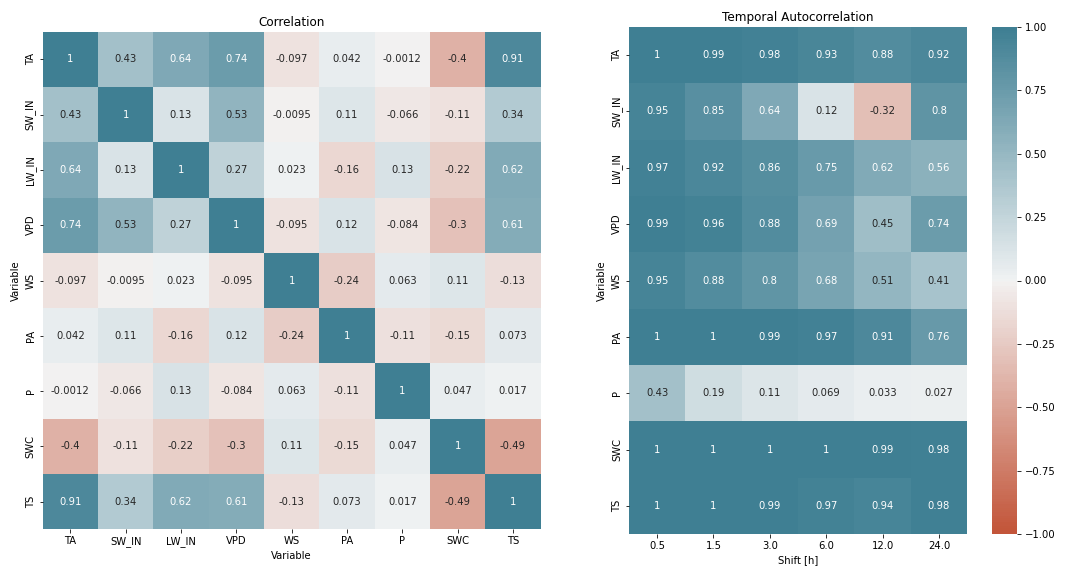
\includegraphics[width=\textwidth]{correlation}

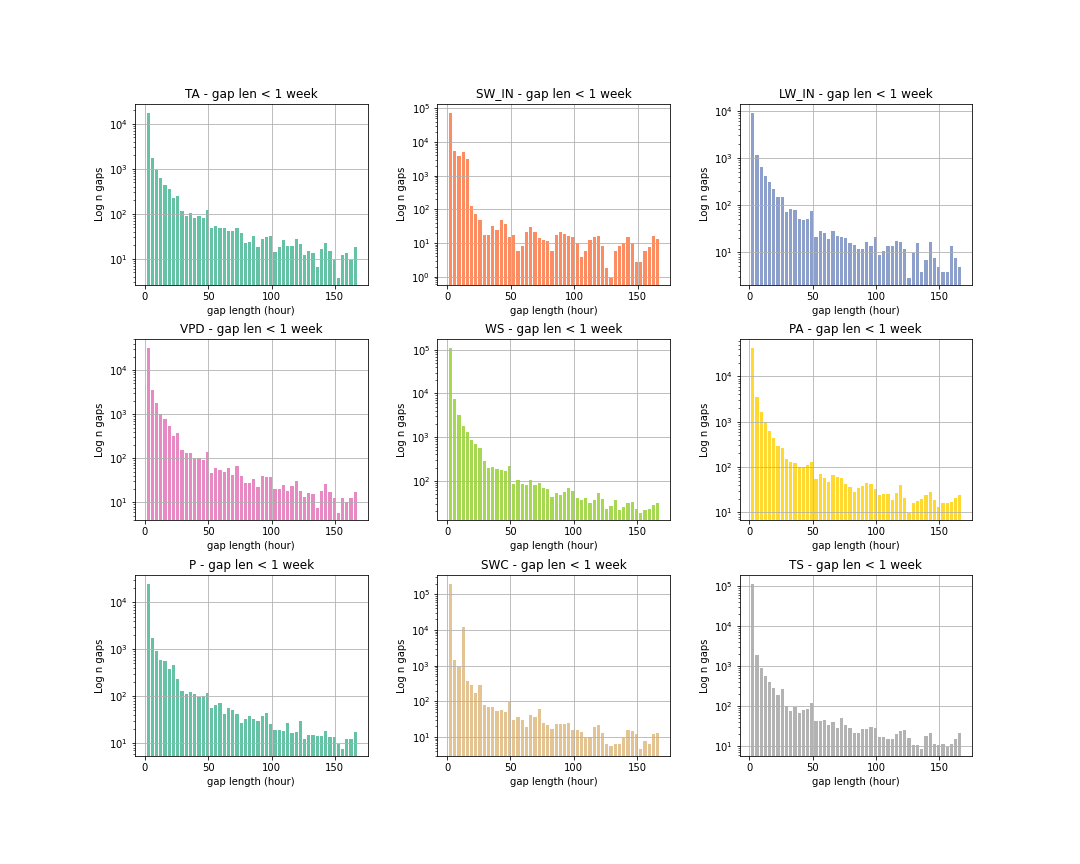
\includegraphics[width=\textwidth]{gap_len_dist_small}

\subsection{Comparison state of art}

\begin{itemize}
    \item 
\end{itemize}

\begin{figure}
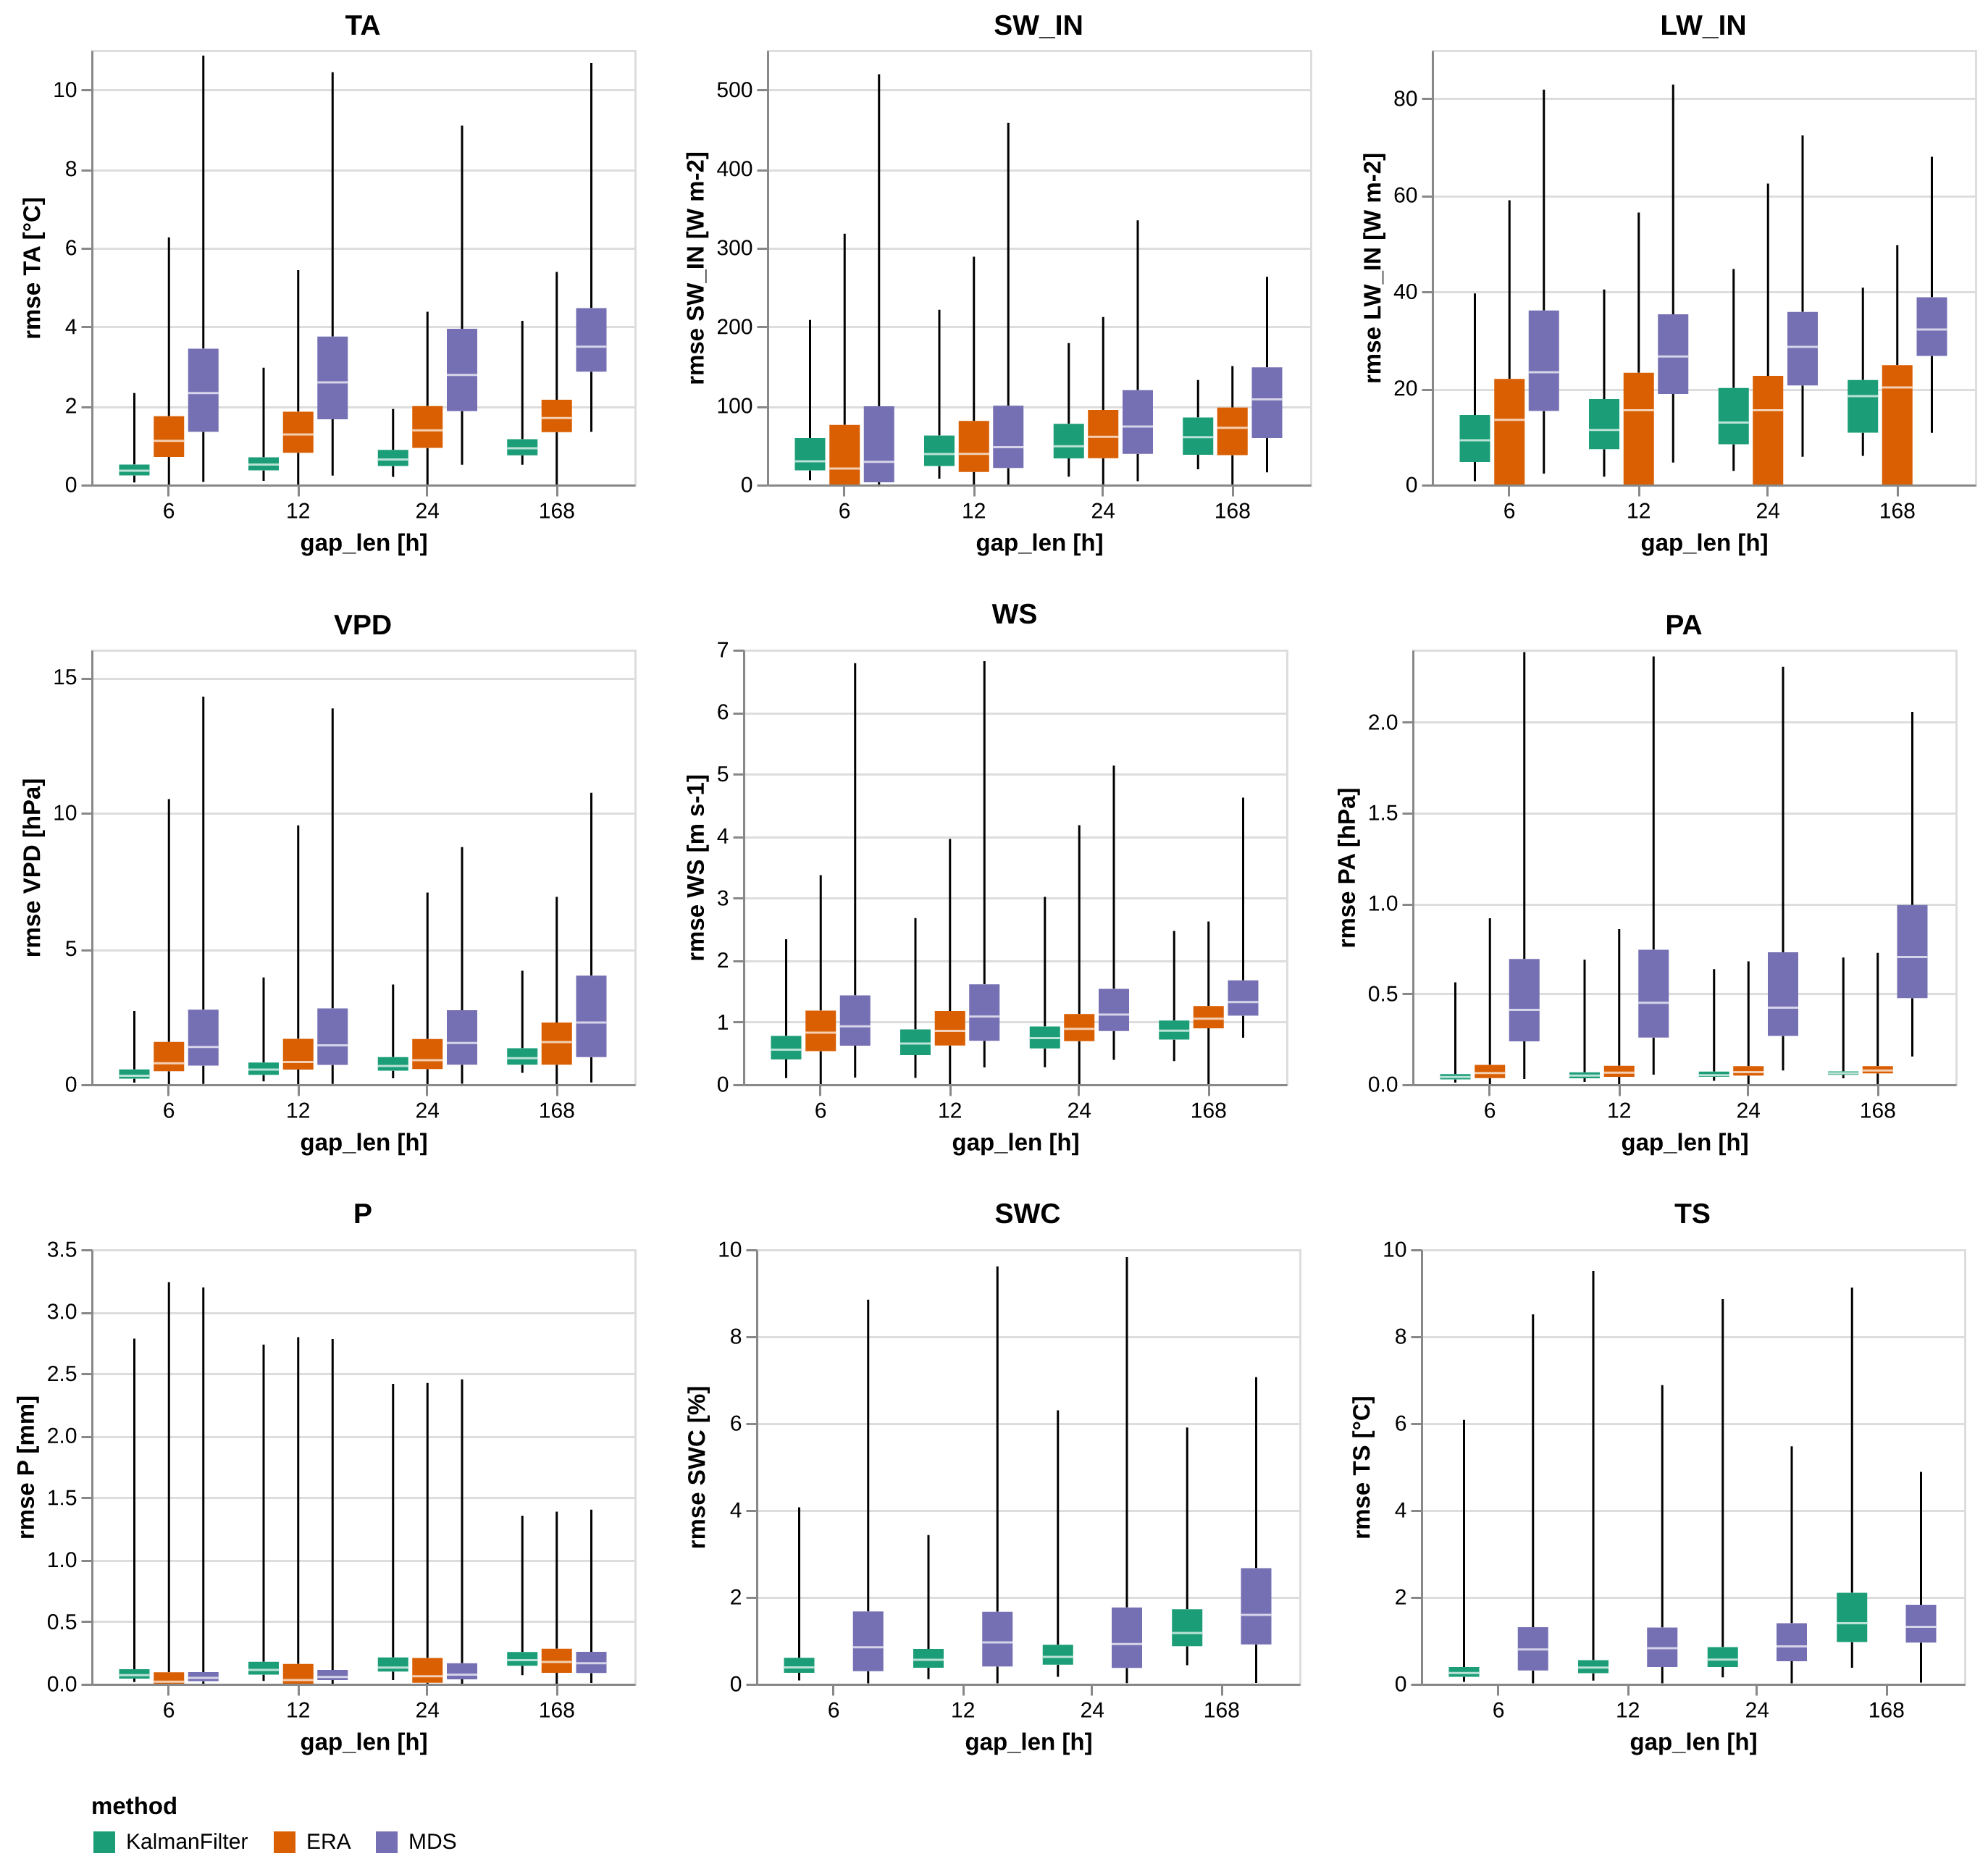
\includegraphics[width=\textwidth]{images/the_plot.png}
\caption{Box plot to compare Root Mean Square Error(RMSE) for each variable between the different methods: Kalman Filter and the state of the art methods ERA and MDS. For each variable and each gap length a artificial gap has been made only in the variable of interest and the gap imputed using the different methods. For each settings }
\end{figure}


\begin{table}
\centering
\caption{RMSE Comparison imputation methods. The best method for each gap length is highligthed in bold}
\label{the_table}
\begin{tabular}{p{2.1cm}c|rr|rr|rr}
\toprule
 &  & \multicolumn{2}{r}{KalmanFilter} & \multicolumn{2}{r}{ERA} & \multicolumn{2}{r}{MDS} \\
 & RMSE & mean & std & mean & std & mean & std \\
Variable & Gap [$h$] &  &  &  &  &  &  \\
\midrule
\multirow[c]{4}{*}{\parbox{2.1cm}{\textbf{TA} [\si{°C}]}} & 6 & \bfseries 0.510 & 0.335 & 1.443 & 1.030 & 2.624 & 1.677 \\
 & 12 & \bfseries 0.685 & 0.412 & 1.347 & 0.788 & 2.665 & 1.546 \\
 & 24 & \bfseries 0.898 & 0.549 & 1.460 & 0.730 & 3.024 & 1.717 \\
 & 168 & \bfseries 1.078 & 0.561 & 1.765 & 0.714 & 3.803 & 1.232 \\
\cline{1-8}
\multirow[c]{4}{*}{\parbox{2.1cm}{\textbf{SW\_IN} [\si{W/m^2}]}} & 6 & 42.053 & 36.503 & \bfseries 41.878 & 57.449 & 56.796 & 79.190 \\
 & 12 & \bfseries 49.334 & 33.321 & 51.587 & 48.850 & 63.173 & 63.886 \\
 & 24 & \bfseries 54.067 & 26.651 & 61.879 & 38.392 & 86.693 & 63.036 \\
 & 168 & \bfseries 59.130 & 24.263 & 66.392 & 33.962 & 99.610 & 53.139 \\
\cline{1-8}
\multirow[c]{4}{*}{\parbox{2.1cm}{\textbf{LW\_IN} [\si{W/m^2}]}} & 6 & \bfseries 11.647 & 8.194 & 14.299 & 13.000 & 27.309 & 15.357 \\
 & 12 & \bfseries 14.098 & 8.483 & 15.719 & 12.606 & 29.660 & 14.269 \\
 & 24 & \bfseries 13.846 & 7.289 & 13.970 & 11.779 & 29.612 & 13.066 \\
 & 168 & 16.756 & 6.761 & \bfseries 15.921 & 11.370 & 32.895 & 8.250 \\
\cline{1-8}
\multirow[c]{4}{*}{\parbox{2.1cm}{\textbf{VPD} [\si{hPa}]}} & 6 & \bfseries 0.575 & 0.496 & 1.356 & 1.546 & 2.200 & 2.280 \\
 & 12 & \bfseries 0.897 & 0.749 & 1.352 & 1.497 & 2.027 & 2.192 \\
 & 24 & \bfseries 1.014 & 0.632 & 1.359 & 1.172 & 2.168 & 1.915 \\
 & 168 & \bfseries 1.285 & 0.799 & 1.625 & 1.111 & 2.400 & 1.898 \\
\cline{1-8}
\multirow[c]{4}{*}{\parbox{2.1cm}{\textbf{WS} [\si{m/s}]}} & 6 & \bfseries 0.585 & 0.303 & 0.894 & 0.491 & 1.194 & 0.667 \\
 & 12 & \bfseries 0.702 & 0.343 & 0.956 & 0.595 & 1.279 & 0.808 \\
 & 24 & \bfseries 0.857 & 0.385 & 1.049 & 0.510 & 1.369 & 0.794 \\
 & 168 & \bfseries 0.912 & 0.278 & 1.063 & 0.322 & 1.454 & 0.508 \\
\cline{1-8}
\multirow[c]{4}{*}{\parbox{2.1cm}{\textbf{PA} [\si{hPa}]}} & 6 & \bfseries 0.052 & 0.068 & 0.077 & 0.095 & 0.520 & 0.387 \\
 & 12 & \bfseries 0.055 & 0.056 & 0.080 & 0.072 & 0.573 & 0.434 \\
 & 24 & \bfseries 0.057 & 0.029 & 0.078 & 0.043 & 0.550 & 0.406 \\
 & 168 & \bfseries 0.065 & 0.026 & 0.083 & 0.030 & 0.770 & 0.338 \\
\cline{1-8}
\multirow[c]{4}{*}{\parbox{2.1cm}{\textbf{P} [\si{mm}]}} & 6 & \bfseries 0.100 & 0.120 & 0.105 & 0.170 & 0.101 & 0.150 \\
 & 12 & 0.125 & 0.161 & 0.131 & 0.229 & \bfseries 0.119 & 0.193 \\
 & 24 & 0.139 & 0.177 & 0.138 & 0.220 & \bfseries 0.138 & 0.217 \\
 & 168 & \bfseries 0.197 & 0.171 & 0.223 & 0.197 & 0.215 & 0.188 \\
\cline{1-8}
\multirow[c]{4}{*}{\parbox{2.1cm}{\textbf{SWC} [\si{\%}]}} & 6 & \bfseries 0.481 & 0.360 & nan & nan & 1.150 & 1.287 \\
 & 12 & \bfseries 0.605 & 0.395 & nan & nan & 1.380 & 1.629 \\
 & 24 & \bfseries 0.764 & 0.760 & nan & nan & 1.665 & 1.714 \\
 & 168 & \bfseries 1.508 & 0.982 & nan & nan & 2.023 & 1.493 \\
\cline{1-8}
\multirow[c]{4}{*}{\parbox{2.1cm}{\textbf{TS} [\si{°C}]}} & 6 & \bfseries 0.403 & 0.457 & nan & nan & 0.983 & 1.113 \\
 & 12 & \bfseries 0.613 & 0.764 & nan & nan & 0.975 & 0.844 \\
 & 24 & \bfseries 0.853 & 0.767 & nan & nan & 0.977 & 0.817 \\
 & 168 & \bfseries 1.358 & 0.697 & nan & nan & 1.507 & 0.829 \\
\cline{1-8}
\bottomrule
\end{tabular}
\end{table}


\subsubsection{Example Time series}

\textbf{goal} Show how a Kalman Filter Gap filling looks like and the uncertainty 

\includegraphics[width=\textwidth]{timeseries}

\begin{itemize}
    \item a few sample variables (max 3/4)
    \item a representative gap length
    \item manually choose interesting gaps (2-4)
    \item no gap in other variable
\end{itemize}

This is the most intuitive way of looking at gap filling and can select the gaps for highlighting the strengths and weakness of the filter


\subsection{Analysis Kalman Filter}

\subsubsection{Gap Length}

\textbf{goal} impact of the gap length on the gap filling

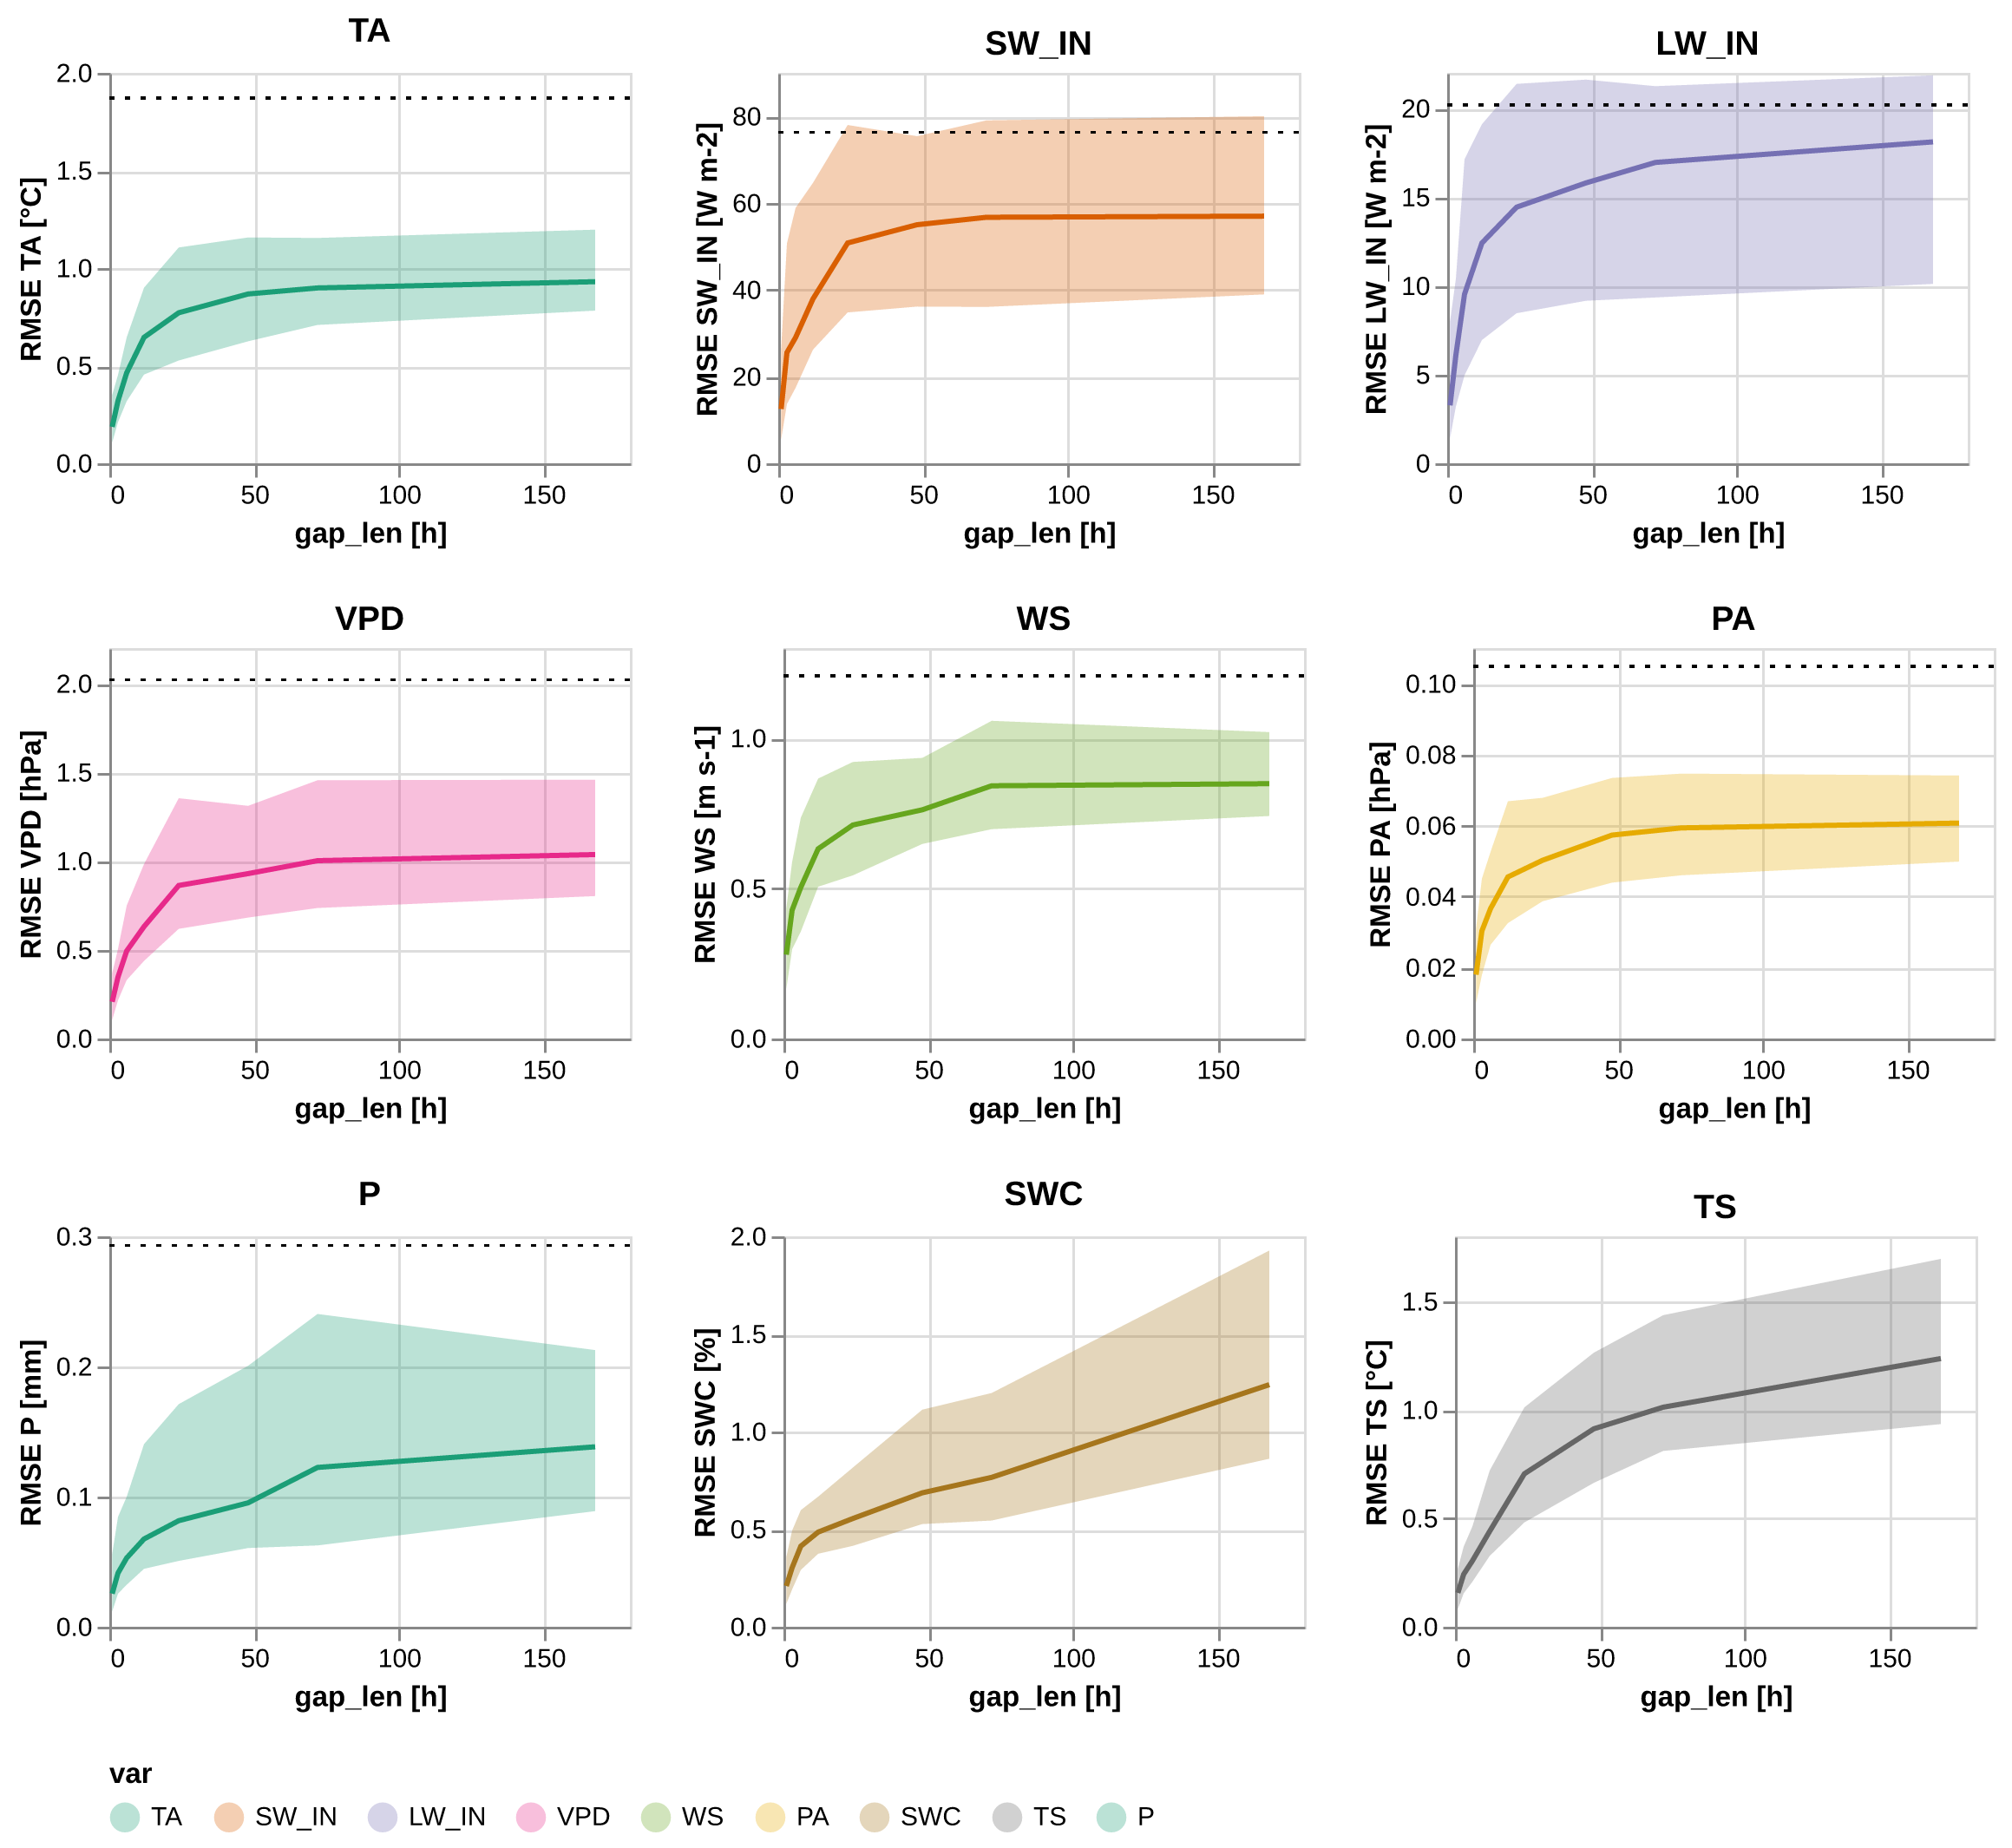
\includegraphics[width=\textwidth]{gap_len}

+ table appendix

\subsubsection{Gap other variable}

\includegraphics[width=\textwidth]{gap_other_vars}

+ table appendix

\subsubsection{Control variable}

\textbf{goal} show how the use of the control (ERA-5 data) in the gap is impacting the predictions

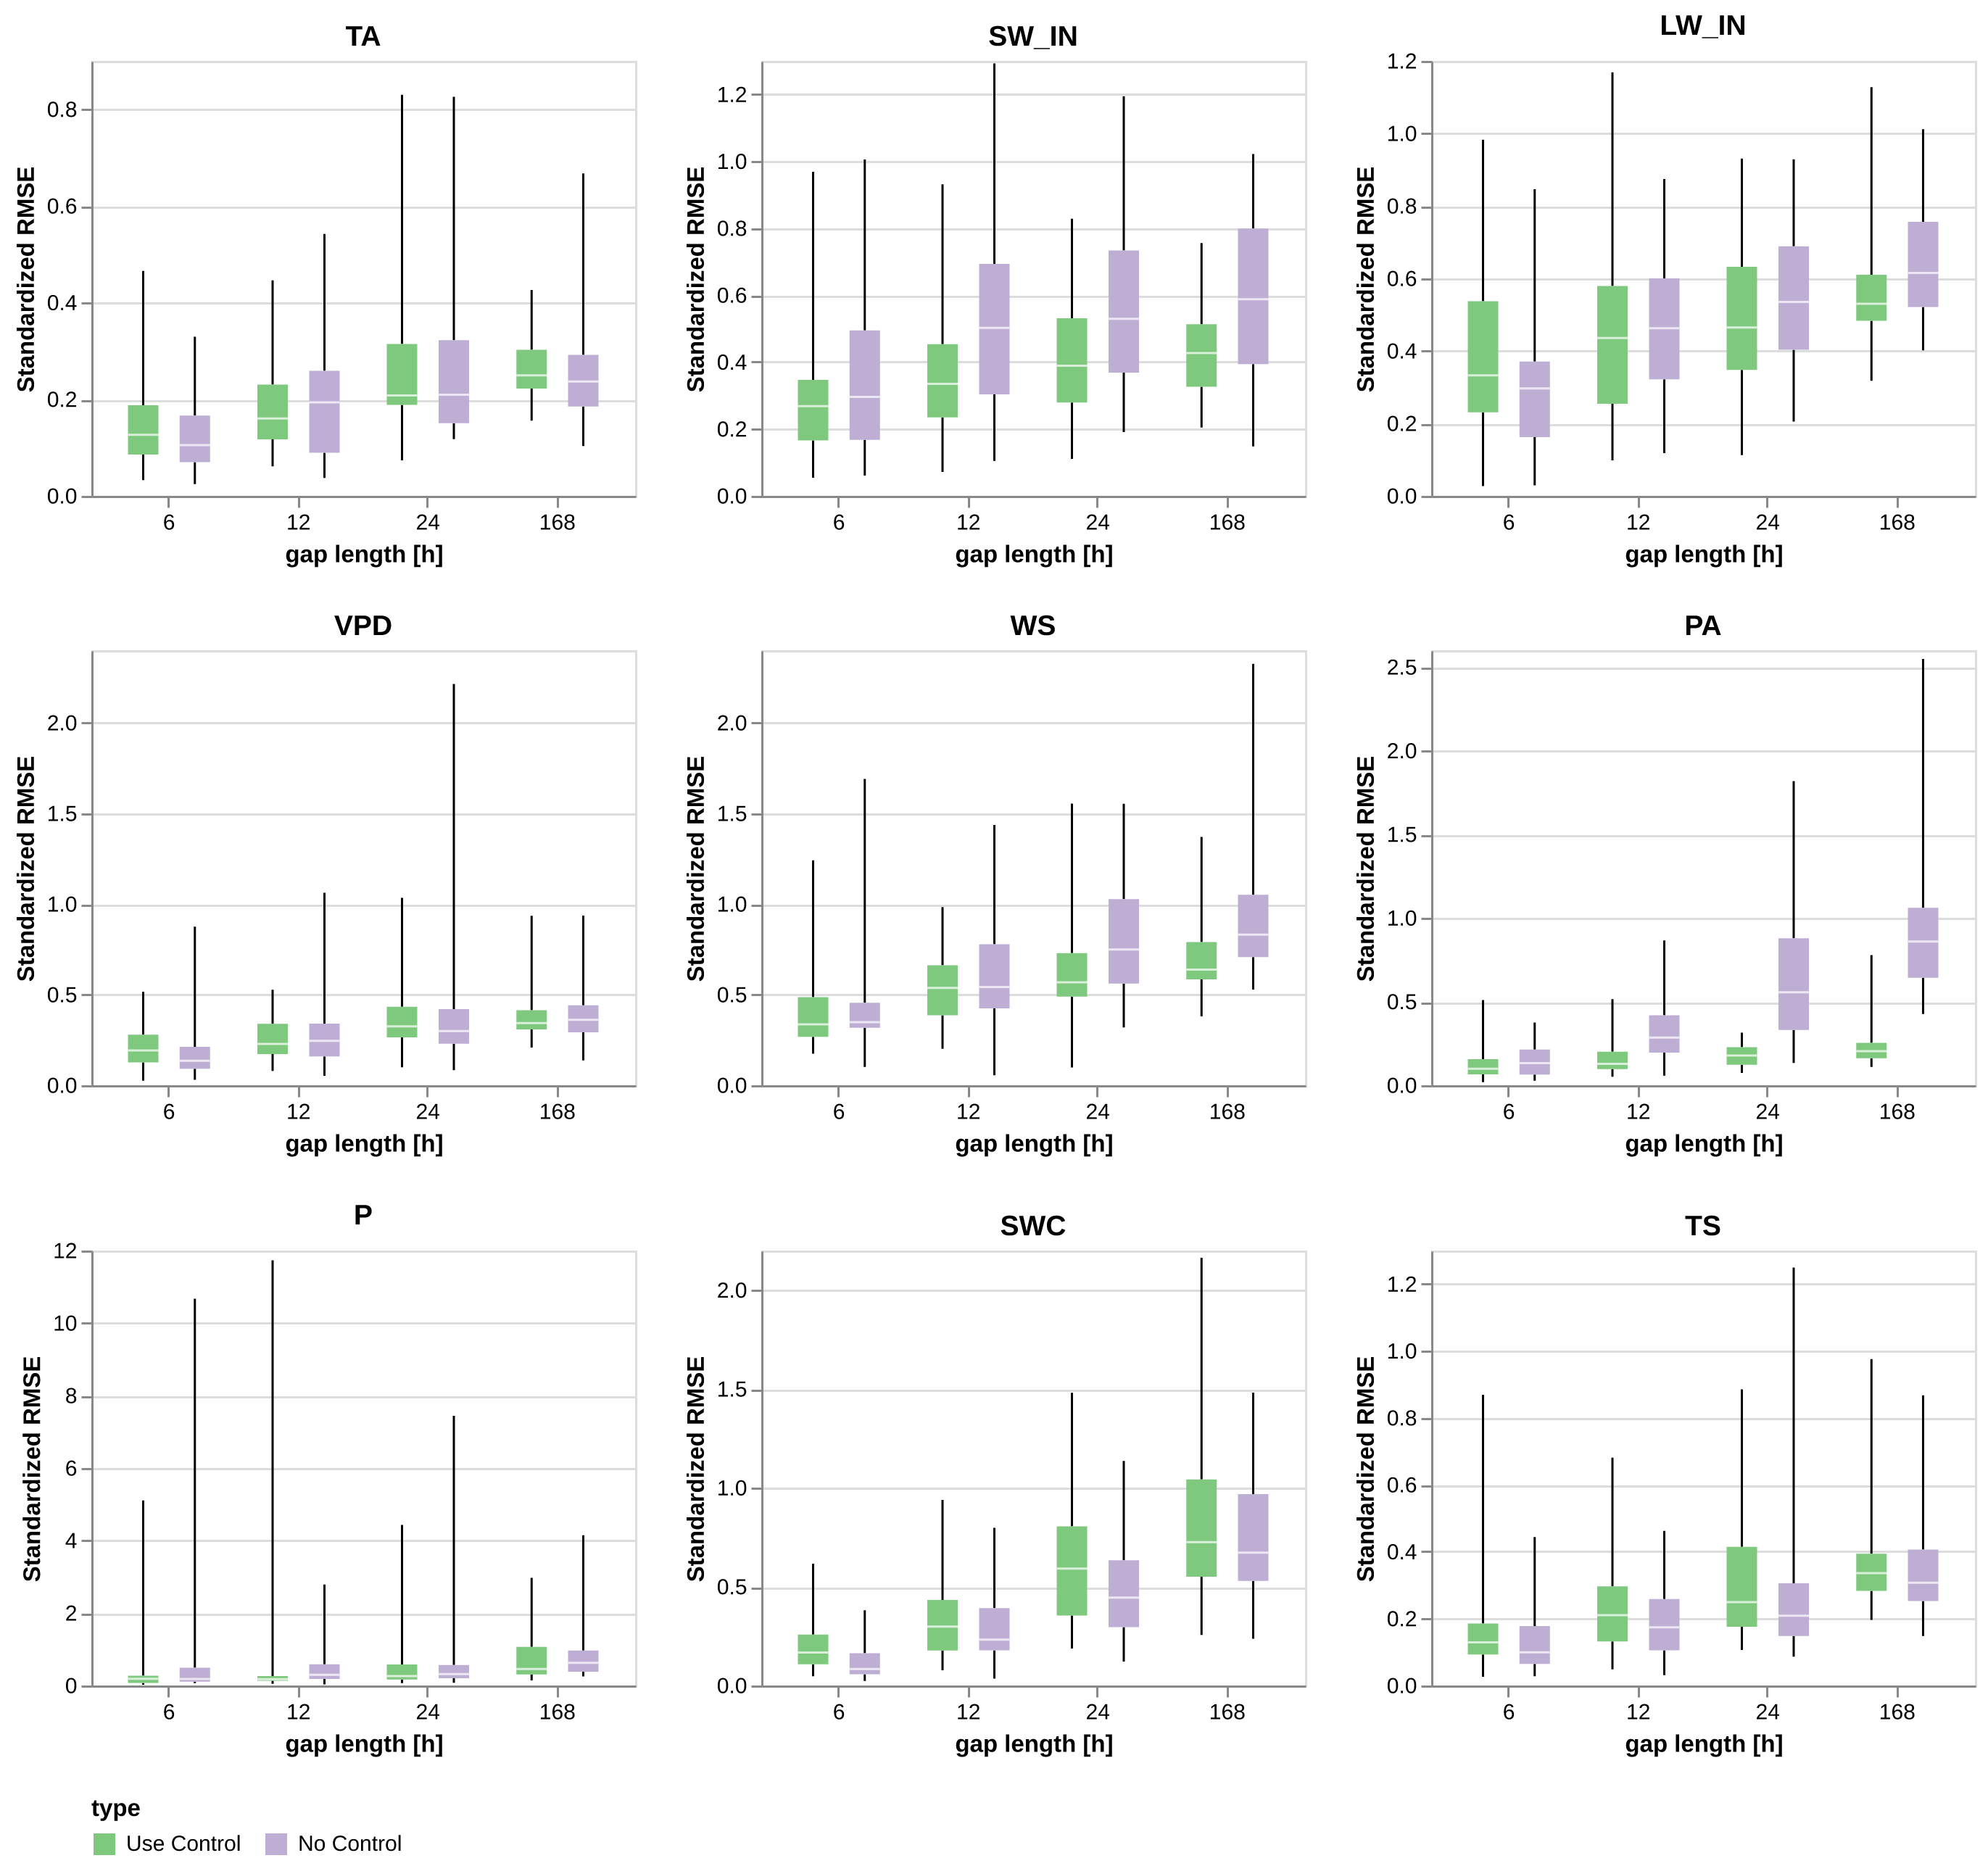
\includegraphics[width=\textwidth]{use_control}

+ table appendix


\subsubsection{Specialized model}

% \includegraphics[width=\textwidth]{specialized}

+ table appendix


\section{Discussion}

\subsection{Comparison other methods}

\begin{itemize}
    \item Kalman Filter works much better than MDS as it can use observation before/after
    \item overall low correlation between meteo variables -> MDS is limited
    \item more precise than ERA as uses local conditions
    \item problem with precipitation
    \item SW IN poor performance?
\end{itemize}

\subsection{Kalman Filter Components}

\begin{itemize}
    \item as expected the longer gap length the worse the performance
    \item the standard deviation of the increases with gap len
\end{itemize}

\begin{itemize}
    \item the presence of other variables in the gap doesn't help a lot for gap filling
    \item exception is TA and LW IN, which have higher correlation
    \item control ?
\end{itemize}


\subsection{Impact of numerical stability}

\begin{itemize}
    \item max gap len is 15 hours model can be trained
    \item Kalman filter is a local model, so for long gaps can't really use it
    \item still need to work to improve numerical stability which should make this better (see appendix)
\end{itemize}


\subsection{Future steps}

\subsubsection{data}
\begin{itemize}
    \item train model for different sites and see difference between sites
    \item use ERA-5 Land data
\end{itemize}

\subsubsection{Gap filling quality assessment}

\begin{itemize}
    \item can train with more realistic gaps properties (length/other variables missing/time of day)
    \item better analysis of gaps in fluxnet
\end{itemize}

\subsubsection{Model improvement}

\begin{itemize}
\item numerical stability
\item make a model to predict the parameters of the Kalman Filter depending on the conditions
\item use Neural Network to process control variable
\end{itemize}



\section{Conclusions}



\section*{References}

\printbibliography

\appendix

\section{Detaild Notation}

\begin{itemize}
\item $t$  Number of time steps
\item observations
\begin{itemize}
    \item $n$  Number of variables observed
    \item $y_{:,t}$ or $y_t$ vector of all the $n$ variables at time $t$, $\in \mathbb{R}^n $
    \item $y_{n,:}$ vector of the $n$th variable at for time steps in $t$, $\in \mathbb{R}^T$
    \item $y_{n,t}$ $n$th variable at time $t$, $\in \mathbb{R}$ 
    \item $Y_M = [x_{:,1}, ... x_{:, t}]$ Matrix with all the $n$ variables at all time steps, $\in \mathbb{R}^{n \times t}$ 
    \item $Y$ is a vector obtained by "flattening" $X_M$, by putting next to each other all variable at time $t$, $\in \mathbb{R}^{(n \cdot t)}$
    \item $y^{ng}_t$ vector of variable that are not missing (ng = not gap)) at time $t$, $\in \mathbb{R}^{n_{ng}}$. Note at different times the shape of this vector can change
    \item $Y^{ng}$ all observations
\end{itemize}

\item Latent state
\begin{itemize}
    \item $k$  Number of variables in latent state
    \item $x_{:,t}$ or $x_t$ vector of all the $k$ state variables at time $t$, $\in \mathbb{R}^k $
    \item $x_{k,:}$ vector of the $k$th variable at for time steps in $t$, $\in \mathbb{R}^t$
    \item $x_{k,t}$ $k$th variable at time $t$, $\in \mathbb{R}$ 
    \item $X_M = [x_{:,1}, ... x_{:, t}]$ Matrix with all the $k$ variables at all time steps, $\in \mathbb{R}^{k \times t}$ 
    \item $X$ is a vector obtained by "flattening" $X_M$, by putting next to each other all variable at time $t$, $\in \mathbb{R}^{(k \cdot t)}$
\end{itemize}

\end{itemize}

\section{Fluxnet gaps}

\section{Comparison Standard Square Root Kalman Filter}

\subsection{Numerical Stability}

\begin{figure}
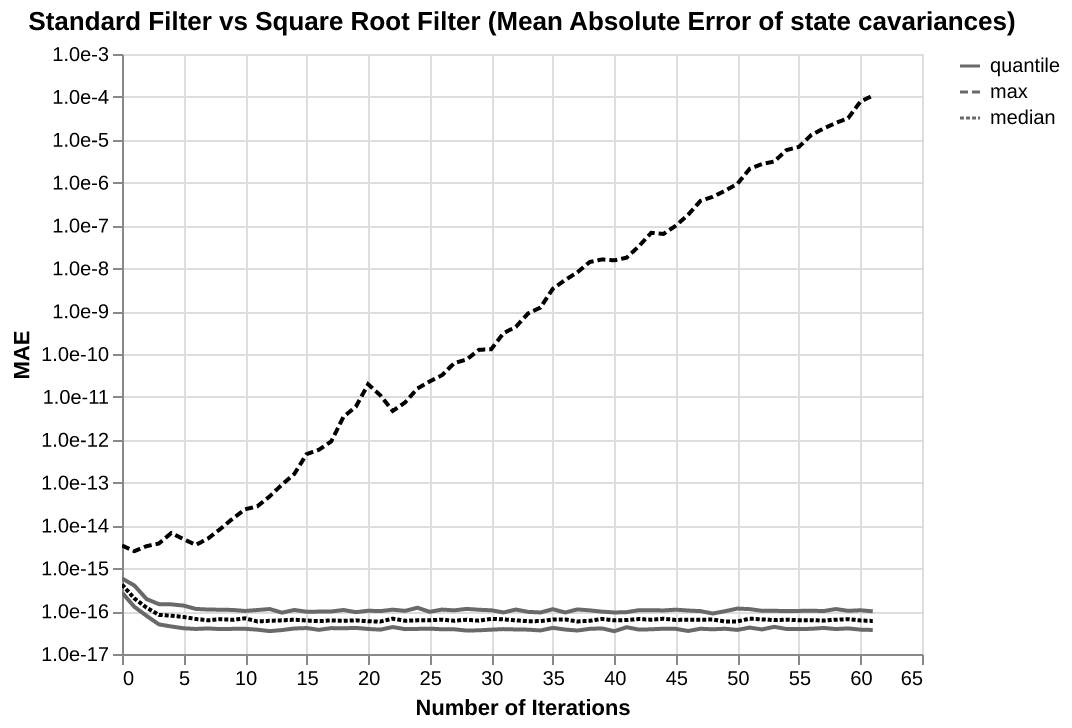
\includegraphics[width=\textwidth]{numerical_stability}
 \caption{Comparison of standard Kalman Filter implementation and Square Root Filter. For 100 times the filter has been initialized with random parameters (drawn from a uniform distribution range 0-1) and then filtered 62 observations. At each filter iteration calculated the Mean Absolute Error (MAE) between the state covariance from the standard filter and the square root filter. The plot shows the median, 1 and 3 quartile and the maximum of the MAE across the 100 samples. You can see that usually the two filter implementations agree, but for a few parameters combinations the error is growing with the number of iterations of the filter suggesting a numerical stability issue. After 62 iterations the standard filter crashes because the covariance is not positive definite anymore. The initial bigger error can be explained by the slightly different initial state covariance.}
\end{figure}


\section{Proofs}

\subsection{Proof for eigenvalues of $CC^T$}

The eigenvalues of the transpose of a matrix are the same of the eigenvalues of a matrix

The properties of the eigenvalues is that $Ax=\lambda x$ for any vector $x$

Then $CC^Tx=C(\lambda x) = \lambda Cx = \lambda^2 x$

\subsection{UD Filter}


This is not relevant anymore, keeping this for now

The UD filter (\cite{bierman_numerical_1977}) is named after the $UDU^T$ decomposition\footnote{In the literature $U$ is a lower \textbf{unit} triangular matrix, but the PyTorch routine just makes lower triangular matrices. In my understanding this makes no difference in the derivation of the equations}, which is also known as the $LDL^T$ decomposition (\cite{golub_matrix_2013}) and it always exists for a positive definite matrix. Where $U$ is a lower triangular matrix and $D$ is a diagonal matrix.

The UD Filter never computes the state covariance matrix $P$, but propagates the $U$ and $D$ components of the matrix to improve the numerical stability. Hence, the filter equations need to be rewritten by using only the $U$ and $D$ components and never the $P$ matrix

\subparagraph{Measurement update}

After each observation at time $t$ the state covariance is updated according to equation \ref{filter_correct}, which is here repeated (for notation simplicity the time subscripts are removed):

$$ P = P^- - P^-H^T(HP^-H^T + R)^{-1}HP^-$$

The goal is to obtain the $U$ and $D$ factors of $P$ given the $U^-$ and $D^-$ factors of $P^-$.

Letting:
\begin{itemize}
    \item $P = UDU^T$
    \item $P^- = U^-D^-U^{-T}$, with $U^{-T}$ being the transpose of $U^-$ not the transpose of the inverse of $U$
    \item $v = U^{-T}H^T$
\end{itemize}
then 
\begin{align}
    &UDU^T = \\
    &= U^-D^-U^{-T} - U^-D^-U^{-T}H^T\left(HU^-D^-U^{-T}H^T + R\right)^{-1}HU^-D^-U^{-T} \\
    &= U^-\left[D^- - D^-v(v^TD^-v+R)^{-1}v^TD^- \right]U^{-T}
\end{align}

If you do a UD decomposition of $\left[D^- - D^-v(v^TD^-v+R)^{-1}v^TD^- \right] = BDB^T$, where $B$ is a lower triangular matrix and $D$ is a diagonal matrix, then 

\[ UDU^T = U^-(BDB^T)U^{-T} = (U^-B)D(U^-B)^{T}) \]

$D$ is the diagonal factor of $P$ as and $U$ is equal to $U^-B$, since $U^-B$ is a lower triangular matrix as is the products of two lower triangular matrices.

Therefore, to perform the measurement update step it is necessary to compute the $UDU^T$ decomposition of $\left[D^- - D^-v(v^TD^-v+R)^{-1}v^TD^- \right]$, which can be implemented using the \verb|torch.linalg.ldl_factor| function.

\subparagraph{Time update}

The state covariance at time $t$ is obtained from the state at time $t-1$ according to the equation \ref{filter_predict}, which is here repeated:

$$ P_t = AP_{t-1}A^T + Q$$

The goal is to obtain the $U_t$ and $D_t$ factors of $P_t$ given the $U_{t-1}$ and $D_{t-1}$ factors of $P_{t-1}$.

Letting:

\begin{align}
    Q &= GD_QG^T\\
    W &= \begin{bmatrix}AU_{t-1}&G\end{bmatrix}\\
    D_w &= \begin{bmatrix}D_{t-1} & 0 \\ 0& D_Q \end{bmatrix}
\end{align}

where $D_Q$ is diagonal and $G$ is lower triangular (the UD decomposition of Q), then:

\begin{equation}
\begin{split}
   P &= WD_wW^T = \\
&=\begin{bmatrix}AU_{t-1}&G\end{bmatrix}\begin{bmatrix}D_{t-1} & 0 \\ 0& D_Q \end{bmatrix}\begin{bmatrix}U^T_{t-1}A^T\\G^T\end{bmatrix} \\
&= AU_{t-1}D_{t-1}U^T_{t-1}A^T + GD_QG^T  
\end{split}
\end{equation}

Then if we can find decompose $W$ as matrices $U_tV$ where $U_t$ is a lower triangular matrix such as that $VD_wV^T$ is a diagonal matrix then

\begin{equation}
    P_t = (U_tV)D_w(U_tV)^T = U_tD_tU_t
\end{equation}

so we have the $U_t$ and $D_t$ factors of $P_t$

This decomposition can be efficiently implemented in PyTorch using some modifications of the QR decomposition \footnote{\url{https://pytorch.org/docs/stable/generated/torch.linalg.qr.html}}

\subsubparagraph{PyTorch Implementation}

The QR decomposition in PyTorch  decompose a matrix $A = QR$, where $Q$ is an orthogonal matrix and $R$ is an upper triangular matrix.
However, for the filter there are two changes that needs to be made:
\begin{enumerate}
    \item decompose into the product of the lower triangular matrix and a diagonal matrix $A = LQ$
    \item have a weighted decomposition regarding a matrix $D$, such as that $QDQ^T = I$ instead of $QQ^T = I$
\end{enumerate}

\sssparagraph{1) Lower triangular matrix}

To obtain a lower triangular matrix from the $QR$ decomposition, you can compute the QR decomposition of $A^T=QR$ and then $A = R^TQ^T$ where $R^T$ is a lower triangular matrix and $Q^T$ is still an orthogonal matrix.

\sssparagraph{2) Weighted decomposition}

The QR decomposition can be used to have a weighted decomposition \footnote{\url{https://scicomp.stackexchange.com/a/33436}}, where $QDQ^T = I$ instead of the $QQ^T = I$.
If $D$ is positive definite, it is possible to apply the Cholesky decomposition of $D = CC^T$. Then you can compute the QR factorization of $CA=UR$, where $U$ is an orthogonal matrix and $R$ is an upper triangular matrix. Then can define $Q=C^{-1}U$. This can be proved as 
$Q D Q^T = C^{-1}U CC^TU^T(C^{-1})^T= I$
In the filter context $D$ is a diagonal matrix computing so the Cholesky decomposition can be efficiently done by taking the square root of every element.

\sssparagraph{Summary} $W$ can be decomposed as $W=U_tV$ with the following procedure:

$$(C_{D_W}W)^T = QR$$ using \verb|torch.linalg.qr| and then defining $U_t = R^T$ and $V=C_{D_W}^{-1}Q^T$

\section{Joint log likelihood}

\subsubsection{Joint distribution of the gap}

The goal is to obtain the joint distribution of the variables in the gap $Y^g$, which is $[y^g_t, y^g_{t+1} ... y^g(t+t_g)]$
for a gap that goes from $t$ to $t+t_g$. $Y^g \in \mathbb{R}^{t_g \times n_g}$, where $n_g$ is the number of variables missing in the gap.

For simplicity we are assuming for now that during the gap the variables missing don't change.

The goal is to obtain $p(Y^g|Y^ng)$

From the Kalman smoother it's easy to obtain $p(y^g_t|Y^{ng}) = \mathcal{N}(\mu_{t}, \Sigma_{t})$

However, the problem is that $y^g_t$ and $y^g_{t+1}$ are not independent so it gets more complex.
Assuming that $p(y^g_t|y^g_{t+1}) = \mathcal{N}(\mu_{t,t+1}, \Sigma_{t,t+1})$ the joint distribution has the form:

$$ p(Y^g|Y^{ng}) = \mathcal{N}\left(\begin{array}{c}
     \mu_{t}   \\
     \mu_{t+1} \\
     \cdots    \\
     \mu_{t+t_g}
\end{array},
\begin{array}{cccc}
    \Sigma_{t}       & \Sigma_{t,t+1}     & \cdots & \Sigma_{t,t+t_g}   \\
    \Sigma_{t+1,t}   & \Sigma_{t+1}       & \cdots & \Sigma_{t+1,t+t_g} \\
    \vdots           & \vdots             & \ddots & \cdots             \\ 
    \Sigma_{t+t_g,t} & \Sigma_{t+t_g,t+1} & \cdots & \Sigma_{t+t_g}     \\
\end{array}\right)$$


$p(Y_g|Y_{ng}) = \int p(Y_g|X_g)p(X_g|Y)dX_g$


\subsubsection{Joint distribution state for gaps}

\paragraph{Two states}

For simplicity, I am starting with the joint distribution of the filter on a gap where there are no observations and are interested only on the joint distribution of two consecutive states.
The aim is to find $p(x_t, x_{t+1}\mid x_t, Y_{1:t})$

The starting point is:
\begin{itemize}
    \item $x_{t+1} = Ax_{t} + \varepsilon_{t+1}$
    \item $p(x_t \mid Y_{1:t}) = \norm{x_t}{m_t}{P_t}$
    \item $p(\varepsilon_t) = \norm{\varepsilon_t}{0}{Q}$
\end{itemize}

Since all distributions are Gaussian, the joint distribution is also Gaussian


\begin{multline}\label{p_X2_start}
p(x_t, x_{t+1}|x_t) = \norm{\begin{bmatrix}x_t\\x_{t+1}\end{bmatrix}}{\begin{bmatrix}m_t\\Am_t\end{bmatrix}}{\Sigma_{x_t, x_{t+1}}} \\
\Sigma_{x_t, x_{t+1}} = \begin{bmatrix}\E{(x_t-\mu_{x_t})(x_t-\mu_{x_t})^T)}&\E{(x_t-\mu_{x_t})(x_{t+1}-\mu_{x_{t+1}})^T}\\\E{(x_{t+1}-\mu_{x_{t+1}})(x_{t}-\mu_{x_{t}})^T}&\E{(x_{t+1}-\mu_{x_{t+1}})(x_{t+1}-\mu_{x_{t+1}})^T}\end{bmatrix}
\end{multline}

we can compute the covariance using the expectation operator and its properties.

\subparagraph{Second element on the diagonal}

\begin{equation}\label{eq:cov_x_t1_x_t1}
\begin{split}
    &\E{(x_{t+1}-\mu_{x_{t+1}})(x_{t+1}-\mu_{x_{t+1}})^T} =\\
    &=\E{(Ax_t + \varepsilon_{t+1} - Am_t)(Ax_t + \varepsilon_{t+1}- Am_t)^T} =\\
    &= \E{(A(x_t - m_t) + \varepsilon_{t+1})(A(x_t - m_t) + \varepsilon_{t+1})^T} =\\
    &=\E{A(x_t-m_t)(x_t-m_t)^TA^T + \varepsilon_{t+1}(x_t-m_t)^TA^T + A(x_t-m_t)\varepsilon_{t+1}^T + \varepsilon_{t+1}\varepsilon_{t+1}^T} =\\&=\E{A(x_t-m_t)(x_t-m_t)^TA^T} + \E{\varepsilon_{t+1}(x_t-m_t)^TA^T} + \E{A(x_t-m_t)\varepsilon_{t+1}^T} + \E{\varepsilon_{t+1}\varepsilon_{t+1}^T} =\\
    &=A\E{(x_t-m_t)(x_t-m_t)^T}A^T + 0 + 0 + \E{\varepsilon_{t+1}\varepsilon_{t+1}^T} = \\
    &=AP_tA^T + Q
\end{split}
\end{equation}

\subparagraph{off-diagonal element}

\begin{equation}\label{eq:cov_x_t1_x_t}
\begin{split}
    &\E{(x_{t+1}-\mu_{x_{t+1}}) (x_{t}-\mu_{x_{t}}^T} = \E{(Ax_t + \varepsilon_{t+1} -Am_t)(x_t - Am_t)^T} =\\
    &=\E{A(x_t - m_t)(x_t - m_t)^T + \varepsilon_{t+1}(x_t - m_t)^T} =\\&=\E{A(x_t - m_t)(x_t - m_t)^T} + \E{\varepsilon_{t+1}(x_t - m_t)^TA^T} =\\
    &=A\E{(x_t - m_t)^T} + 0 = \\
    &=AP_t
\end{split}
\end{equation}

\subparagraph{Joint distribution state}

substituting in equation \ref{p_X2_start}:

\begin{equation}\label{p_X2_final}
p(x_t, x_{t+1}\mid x_t, Y_{1:t}) = \norm{\begin{bmatrix}x_t\\x_{t+1}\end{bmatrix}}{\begin{bmatrix}m_t\\Am_t\end{bmatrix}}
{\begin{bmatrix}P_t & AP_t\\AP_t & AP_tA^T + Q\end{bmatrix}}
\end{equation}

\paragraph{Multiple States} A similar reasoning can be applied to more than two states, but the equations become more complex

To obtain $p(x_t, x_{t+1}, x_{t+2} \mid x_t, Y_{1:t})$ we also need to compute $\E{x_tx_{t+2}^T}$ and $\E{x_{t+2}x_{t+2}^T}$

\subparagraph{Covariance diagonal}

\begin{equation}\label{eq:cov_x_t_x_t2}
\begin{split}
    &\E{(x_{t+2}-\mu_{x_{t+2}})(x_{t+2}-\mu_{x_{t+2}})^T}=\\
    &= \E{(A(Ax_t + \varepsilon_{t+1}) + \varepsilon_{t+2} - AAm_t)(A(Ax_t + \varepsilon_{t+1}) + \varepsilon_{t+2} - AAm_t)^T} =\\
    &=\E{(AAx_t + A\varepsilon_{t+1} + \varepsilon_{t+2} - AAm_t)(AAx_t + A\varepsilon_{t+1} + \varepsilon_{t+2} - AAm_t)^T}=\\
    &=\E{AA(x_t - m_t)(x_t - m_t)^TA^TA^T} + \E{A\varepsilon_{t+1}\varepsilon{t+1}^TA^T} + \E{\varepsilon_{t+2}\varepsilon_{t+2}^T}=\\
    &=AAP_t(AA)^T + AQA^T + Q
\end{split}
\end{equation}

which (probably) can be generalized as: [TODO actually need to prove this and check that notation is correct]

\begin{equation}
    \E{(x_t -\mu_{x_t})(x_{t+k} - \mu_{x_{t+k}})^T} = A^kP_t(A^k)^T + \sum_{i=0}^{k-1} A^iQ(A^i)^T
\end{equation}

\subparagraph{Covariance off-diagonal}

\begin{equation}
    \E{(x_{t+k} - \mu_{x_{t+k}})(x_{t+k} - \mu_{x_{t+k}})^T} = A^kP_t(A^k)^T
\end{equation}

\subparagraph{Mean}

\begin{equation}
    \E{x_{t+k}} = A^km_t
\end{equation}

\subparagraph{Joint distribution state}
In this way it is possible to obtain $P(X)$ for any number of states.

\begin{multline}\label{p_X_final}
p(X_{t:t+k}\mid x_t, Y_{1:t}) =\norm{\begin{bmatrix}x_t\\\vdots\\x_{t+k}\end{bmatrix}}{\begin{bmatrix}m_t\\\vdots\\A^km_t\end{bmatrix}}{\Sigma_{x_t, x_{t+k}}}\\
\shoveleft\Sigma_{x_t, x_{t+k}} = {\begin{bmatrix}P_t & \cdots & A^kP_t(A^k)^T\\ \vdots & \ddots & \vdots \\A^kP_t(A^k)^T & \cdots & AP_t(A^k)^T + \sum_{i=0}^{k-1} A^iQ(A^i)^T\end{bmatrix}}
\end{multline}



\subsubsection{Joint distribution state - partial observations}

In the case the there are partial observations to the reasoning of the previous paragraph cannot be applied as by combining equations \ref{filter_predict} and \ref{filter_correct_missing}

\begin{equation}\label{filter_combined}
\begin{split}
    m_t^- &= Am_{t-1} + B c_t + d\\
    P_t^- &= AP_{t-1}A^T + Q\\
    z_t &= MHm_t^- + Md\\
    S_t &= MHP_t^-(MH)^T + MRM^T\\
    K_t &= P_t^-(MH)^TS_t^{-1}\\
    m_t &= m_t^- + K_t(My_t - z_t)\\
    P_t &= (I-K_tMH)P_t^-\\
    p(x_t|x_{t-1}, y^{ng}_t) &= \mathcal{N}(x_t; m_t, P_t)
\end{split}
\end{equation}

From this equation is not possible to write $x_t$ and linear map of $x_{t-1}$ plus another random variable, since the mean of $x_t$ depends on the covariance of $x_{t-1}$ 
    
For the same reason this approach cannot be applied for the smoother.

\end{document}

